\documentclass[a4paper]{article}

%%%%%%%%%%%%%%%%%%%%%%%%%%%%%%%%

\usepackage[utf8]{inputenc}
\usepackage[T1]{fontenc}
\usepackage[francais]{babel}
\usepackage{graphicx}
\usepackage{wrapfig}
\usepackage{algorithm2e}
\usepackage{amssymb}
\usepackage{amsthm}
\usepackage{amsmath}
\usepackage{amsfonts}
\usepackage{enumitem}
\usepackage{stmaryrd}
\setlength{\textwidth}{371pt}
\usepackage[all]{xy}
\usepackage{tikz}
\usepackage{titling}
\usepackage{mathtools}
\usepackage{hyperref}
\usepackage{varioref}
\hypersetup{                    % parametrage des hyperliens
    colorlinks=true,                % colorise les liens
    breaklinks=true,                % permet les retours à la ligne pour les liens trop longs
    urlcolor= black,                 % couleur des hyperliens
    linkcolor= black,                % couleur des liens internes aux documents (index, figures, tableaux, equations,...)
    citecolor= black               % couleur des liens vers les references bibliographiques
    }
%%%%%%%%%%%%%%%%%%%%%%%%%%%%%%%%
{\theoremstyle {plain} \newtheorem {definition} {Définition} [section] }
{\theoremstyle {plain}  \newtheorem {theorem} [definition] {Théorème}}
{\theoremstyle {plain}  \newtheorem {prop} [definition] {Proposition}}
{\theoremstyle {plain}  \newtheorem {ex} [definition] {Exemple}}
{\theoremstyle {plain}  \newtheorem {dem} [definition] {Démonstration}}
{\theoremstyle {plain}  \newtheorem {loi} [definition] {Loi de Composition}}
{\theoremstyle {plain}  \newtheorem {lem} [definition] {Lemme}}
{\theoremstyle {plain}  \newtheorem {conj} [definition] {Conjecture}}
{\theoremstyle {plain}  \newtheorem {slem} [definition] {Sous-lemme}}
{\theoremstyle {plain}  \newtheorem {cor} [definition] {Corollaire}}
{\theoremstyle {plain}  \newtheorem {rem} [definition] {Remarque}}
\newcommand{\overbar}[1]{\mkern 1.5m \overline{\mkern-1.5mu#1\mkern-1.5mu}\mkern 1.5mu}
\renewcommand\thesection{\Roman{section}}
\usepackage{mathrsfs}
\usepackage{geometry}
\geometry{hmargin=4cm,vmargin=3cm}
\newtheorem*{preuve}{Preuve du Corollaire}
\newcommand{\eq}[1][r]
   {\ar@<-3pt>@{-}[#1]
    \ar@<-1pt>@{}[#1]|<{}="gauche"
    \ar@<+0pt>@{}[#1]|-{}="milieu"
    \ar@<+1pt>@{}[#1]|>{}="droite"
    \ar@/^2pt/@{-}"gauche";"milieu"
    \ar@/_2pt/@{-}"milieu";"droite"}
%%%%%%%%%%%%%%%%%%%%%%%%%%%%%%%%
\begin{document}

\begin{center}
Universit\'e de Bourgogne \hspace*{\stretch{1}} M1 Mathématiques Approfondies

UFR de Math\'ematiques \hspace*{\stretch{1}} M\'emoire de Master
\end{center}

\vspace*{\stretch{1}} % ressort vertical de force 1

\begin{center}\bfseries\Huge
Les Courbes Elliptiques
\end{center}

\vspace*{1cm} % espace vertical de 1cm

\begin{center}\bfseries\Large
Théophile Hontang
\end{center}
\begin{center}\bfseries\Large
Sous la direction de Ronan Terpereau
\end{center}
\vspace*{\stretch{2}} % ressort vertical de force 2
\begin{center}
Le \today
\end{center}
\newpage
\null
\newpage
\begin{center}
\tableofcontents
\end{center}


\newpage
\section*{Introduction}

Le but de ce mémoire est de présenter les aspects de la théorie des courbes elliptiques.
On a préféré faire une introduction à cette théorie dont le lecteur pourra choisir les parties 
qu'il décidera de lire (un schéma en bas de page représente ces "parcours").
Il est conseillé au lecteur de commencer sa lecture par la première section "Généralités" où est définit la loi de groupe sur les courbes elliptiques, notion cruciale par la suite. \\
La deuxième section porte sur le théorème de Mordell, théorème bien connu des algébristes. La démonstration est longue (six pages) mais elle reste élémentaire, le lecteur peut faire l'impasse sur cette section.
Dans une troisième partie, on présente brièvement les applications en cryptographie très utilisées de nos jours. En annexe, certains algorithmes sont présentés par le logiciel Maple. \\
Pour conclure ce mémoire, on étudie les courbes elliptiques sur $\mathbb{C}$, étude qui aurait pu être un sujet de mémoire à lui seul. Cette partie demande des pré-requis, principalement, en analyse complexe et en théorie des corps. \\
Ce mémoire est influencé par les livres de Joseph H. Silverman\cite{ref},\cite{ref2} et \cite{ref8}, livres conseillés après la lecture de ce mémoire. \\ \\ \\


\begin{figure}[!h]
\begin{center}
\begin{tikzpicture}
% définition des styles
\tikzstyle{quadri}=[rectangle,draw,fill=white!100,text=]
\tikzstyle{estun}=[->,>=latex,very thick,dotted]
% les nœuds
\node[draw] (Q) at (0,3) {Généralités};
\node[draw] (P) at (-3,1) {Théorème de Mordell};
\node[quadri] (R) at (-3,-1.5) {Courbes elliptiques sur $\mathbb{C}$};
\node[quadri] (C) at (4.5,-1.5) {Courbes elliptiques sur $\mathbb{F}_{q}$};
% les flèches
\draw[estun,dashed](Q)--(P);
\draw[->,>=latex] (Q)to[bend left](C);
 \draw[->,>=latex] (P)--(R);
\draw[->,>=latex] (Q)to[bend left](R); \draw[estun,dashed] (P)to[bend left](C);
\draw[->,>=latex] (C)to[bend left](R);
\end{tikzpicture}
\end{center}
\end{figure}

\noindent \textbf{Remerciements}
\\
Je voudrais remercier toutes les personnes qui m'ont aidé dans la réalisation de ce mémoire.
Tout d'abord, je remercie M.Terpereau pour m'avoir guidé tout au long de ces cinq mois. Ensuite, je remercie M.Nagel, M.Faenzi et M.Kitanine pour avoir répondu à mes questions.


\newpage

\section{Généralités}
\subsection{Loi de groupe}
\noindent Soit $\mathbb{K}$ un corps quelconque.
\begin{figure}[h]
\centering
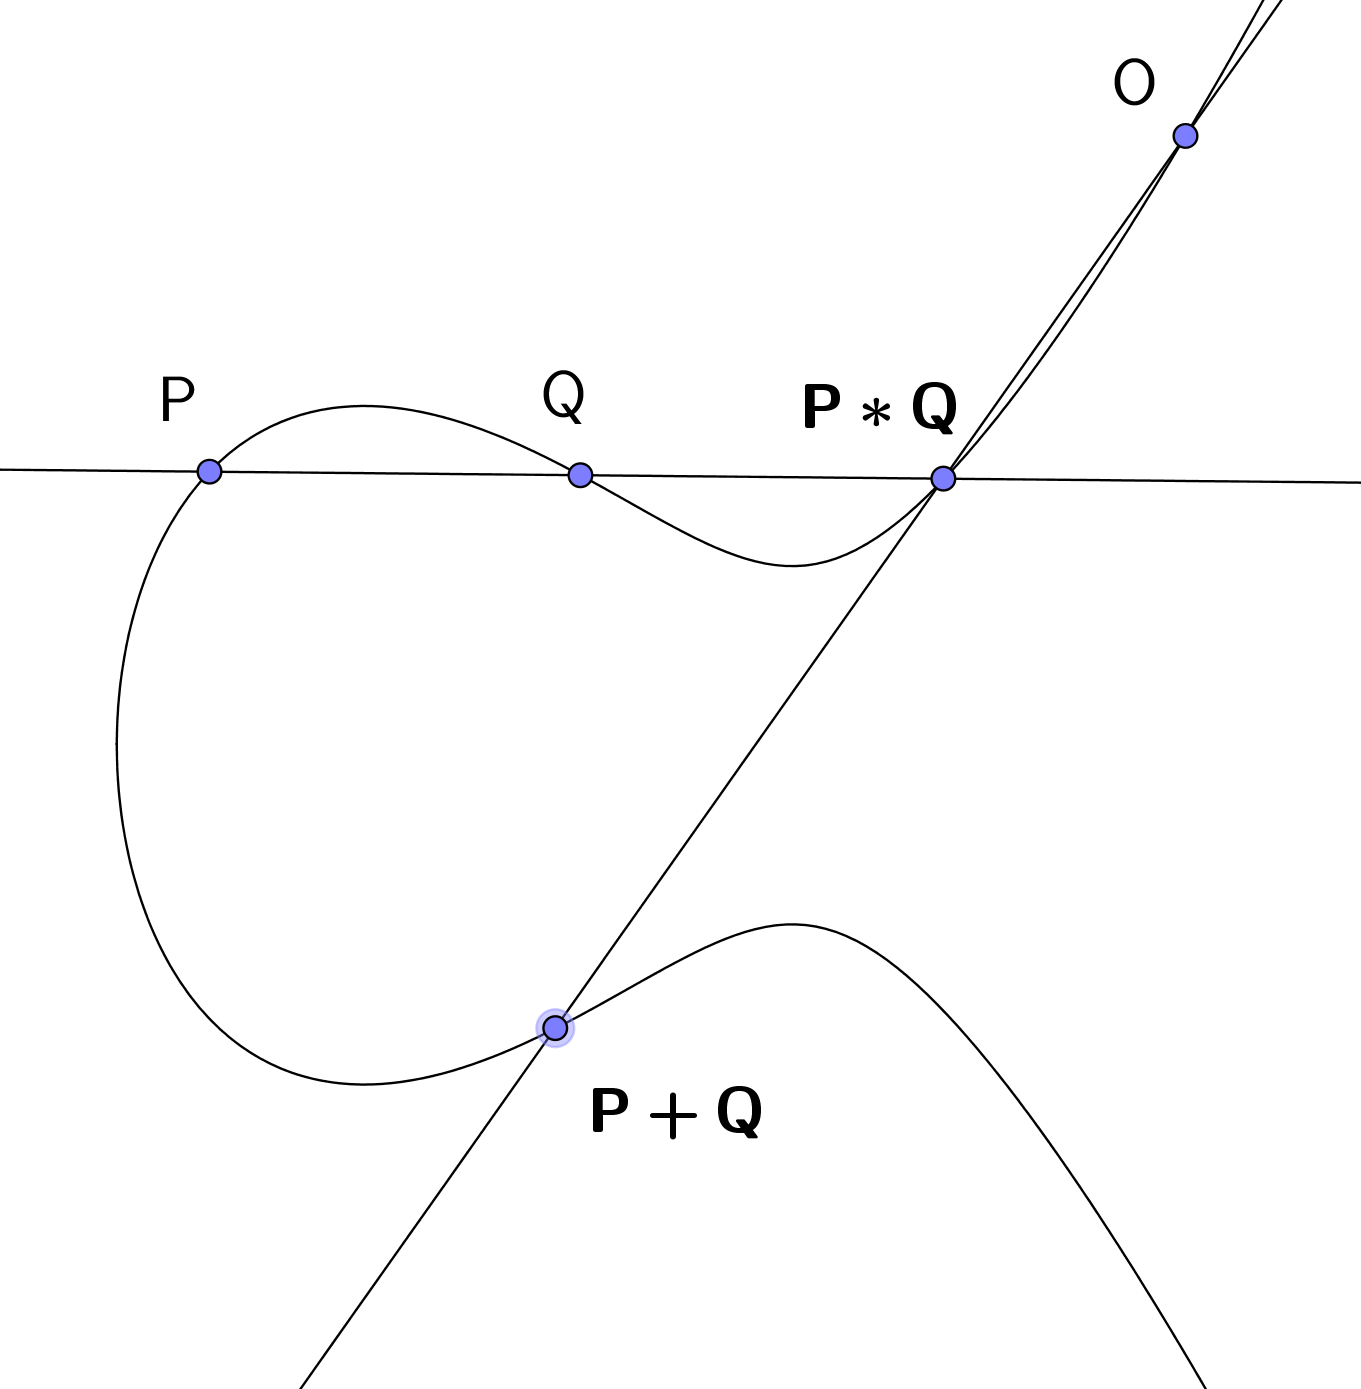
\includegraphics[scale=0.2]{addition.png}
\caption{Loi d'addition}
\label{neutre}
\end{figure} 

\begin{definition}
Dans le plan projectif $\mathbb{P}^2(\mathbb{K})$, $C$ est une \textbf{courbe cubique} sur un corps $\mathbb{K}$ si son équation est $F(X,Y,Z)=0$ où $F(X,Y,Z)$ est un polynôme homogène de degré 3. \\
Si la cubique $C$ est lisse alors on dit que $C$ est une \textbf{courbe elliptique}.
\end{definition}

\begin{rem}
\begin{enumerate}
 \item  Pour les corps de caractéristique différente de 2 et 3, cette équation peut être réduite à 
 \begin{equation*}
 y^2=x^3+ax+b 
 \end{equation*}
 où $a,b \in \mathbb{K}$.
Cette forme n'est pas unique. Les seuls changements de variable préservant cette forme sont : 
\begin{equation*}
x \mapsto u^2x \hspace{1cm} y \mapsto u^3y
\end{equation*}
où $u \in \mathbb{K}$. Nous allons considérer cette forme tout au long du mémoire (sauf mention contraire).
 Voir \cite{ref} pour un exemple.
 \item  En utilisant les coordonnées non homogènes $x=X/Z$ et $y=Y/Z$, nous obtenons 
\begin{equation*}
Y^2 Z=X^3+aXZ^2+b Z^3
\end{equation*}
Cette forme est dite de \textbf{Weierstrass}.
\end{enumerate}
\end{rem}
\noindent Soit $P=(x,y)$ avec $x,y \in \mathbb{K}$. Un des résultats centraux sur les points $P$ des courbes elliptique est le fait qu'ils forment un groupe abélien. Avant de définir la loi de composition du groupe, rappelons le théorème de Bézout (Voir \cite{ref20} pour une démonstration).
\begin{theorem}[Bézout]
Soient $C$ et $C'$ deux courbes projectives planes de degrés $d$ et $d'$ définies sur un corps algébriquement clos, sans composante commune. Alors le nombre de points d'intersection de $C$ et $C'$, comptés avec leurs multiplicités, est égal à $dd'$.
\end{theorem}
\noindent Par le théorème de Bézout, une droite $L$ intersecte $C$ en trois points(Ces points ne sont pas forcément distincts).
Nous allons considérer un point à l'infini, qu'on note $\mathcal{O}$, comme l'ensemble des points $(X:Y:Z) \in C$ tels que
$Z=0$. Cet ensemble est réduit au point $\mathcal{O}=(0:1:0)$.
\\
Définissons la loi de composition $+$ de $C$ par la règle suivante.

\begin{loi}[\cite{ref}]
Soient $P,Q \in C$, la droite $L$ joignant $P$ et $Q$ (ou la tangente si $P=Q$), et $P*Q$ le troisième point d'intersection  de $L$ par $C$.
Soit $L'$ la droite joignant $P*Q$ et $\mathcal{O}$. Alors $P+Q$ est le point tel que $L'$ intersecte $C$ aux points $P*Q$, $\mathcal{O}$ et $P+Q$. C'est à dire:
\begin{equation*}
P+Q=\mathcal{O}*(P*Q).
\end{equation*}
\end{loi}

\begin{prop}[\cite{ref}]
La courbe elliptique $C$, munie de la loi de composition $+$, est un groupe abélien avec $\mathcal{O}$ comme élément neutre.
\end{prop}
\begin{proof} 

Si $Q=\mathcal{O}$, $L$ et $L'$ coïncident. $L$ intersecte $C$ aux points $P,\mathcal{O},R$ et $L'$ intersecte $C$ aux points $P+\mathcal{O},\mathcal{O},R$ d'où $P+\mathcal{O}=P$. \\ 
Si $L$ intersecte $C$ aux points $P,\mathcal{O}$ et un troisième point qu'on note $R$, alors
\begin{equation*}
(P+Q)+R=\mathcal{O}
\end{equation*}
par la définition de loi de groupe.
Nous obtenons 
\begin{equation*}
\mathcal{O}=(P+\mathcal{O})+R=P+R
\end{equation*}
L'associativité est démontré par la figure 5 dans l'annexe. \\
La commutativité provient du fait que la construction de la loi est symétrique en $P$ et $Q$.
\end{proof}
\begin{rem}
\noindent 
Le point $P*Q=(x,y)$ donne le point $P+Q=(x,-y)$, point symétrique par rapport l'axe des abscisses.
Nous remarquons alors que si $P=(x,y) \in C$ alors $-P=(x,-y) \in C$.
\end{rem}
\noindent Dorénavant, nous notons $(C(\mathbb{K}),+)$ ce groupe abélien.


\subsection{Formules de duplication}
\noindent La loi étant définie précédemment, nous pouvons calculer la somme de deux points ou le double d'un point. Ces formules, qu'on nomme \textbf{formules de duplication}, seront utilisées dans les prochaines parties.


\begin{prop}[Formules de duplication \cite{ref}] 
 Soit $C$ une courbe elliptique d'équation $ y^2=x^3+ax^2+bx+c$.
\begin{enumerate}
\item Soient $P_{i}=(x_{i},y_{i}) \in C$ pour $i \in \{1,2\}$.
Alors $P_{1}+P_{2}=(x_{3},y_{3})$ avec 
\begin{equation*}
x_{3}=\lambda^2-a-x_{1}-x_{2} \hspace{1cm} y_{3}=\lambda x_{3}+\nu
\hspace{1cm}
\lambda=\frac{y_{2}-y_{1}}{x_{2}-x_{1}} \hspace{1cm} \nu=y_{1}-\lambda x_{1}
\end{equation*}
\item Soit $P_{0}=(x_{0},y_{0}) \in C$. Alors la coordonnée en $x$ de $2P$ est :
\begin{equation*}
x(2P)=\frac{x_{0}^4-2bx_{0}^2-8cx_{0}+b^2-4ac}{4x_{0}^3+4ax_{0}^2+4bx_{0}+4c}
\end{equation*}
\end{enumerate}
\end{prop}

\begin{proof}
1) Soient $P_{1}*P_{2}=(x_{*},y_{*})$.
La droite joignant $P_{1}$ et $P_{2}$ est définie par l'équation $y=\lambda x+\nu$ avec $\lambda=\frac{y_{2}-y_{1}}{x_{2}-x_{1}}$ et $\nu=y_{1}-\lambda x_{1}$.
L'intersection de cette droite avec $C$ est définie par :
\begin{equation*}
x^3+(a-\lambda^2)x^2+(b-2\lambda\nu)x+(c-\nu^2)=0
\end{equation*}
Les trois racines de ce polynôme sont $x_{1},x_{2}$ et $x_{*}$.
Par les relations de Viète qui expriment les coefficients du polynôme par les racines, nous obtenons :
\begin{equation*}
a-\lambda^2=-(x_{1}+x_{2}+x_{3})
\end{equation*}
Comme $x_{3}=x_{*}$ et $y_{3}=-y_{*}$, nous obtenons bien les coordonnées de $P_{1}+P_{2}$. \\
2) $P*P$ est obtenu par l'intersection de $C$ et de la tangente de $C$ en $P$. La pente est $\lambda={\frac{dy}{dx}}(P_{0})=\frac{f'(x_{0})}{2y_{0}}$. En substituant $\lambda$ dans les équations obtenues en 1) et en remplaçant $y^2$ par $x^3+ax^2+bx+c$, nous obtenons le résultat.

\end{proof}

\subsection{Points d'ordre fini} 
\noindent Nous allons maintenant définir l'ordre d'un élément du groupe $(C(\mathbb{K}),+)$.
\begin{definition}
Pour $n \in \mathbb{Z}$, on définit l'application
\begin{align*}
[n] : C &\rightarrow C \\
P &\mapsto \left\{
    \begin{array}{ll}
        [n]\hspace{0.13cm} P =\underbrace{P+...+P}_{n fois} & \mbox{si }n>0 \\
 \begin{bmatrix} n \end{bmatrix}P  =\begin{bmatrix} -n \end{bmatrix}(-P)  & \mbox{si }  n<0
    \end{array}
\right.
\end{align*}
Si $n=0$ alors $[0]P=\mathcal{O}$. \\
Cette application sera utile pour la section "Multiplication complexe", section IV.4. \\
Un point $P$ est d'ordre fini $n>0$ si $[n]P=\mathcal{O}$ et $[m]P \neq \mathcal{O}$ pour $m<n$.
Sinon $P$ est d'ordre infini.
\end{definition}

\noindent Il existe une caractérisation simple des points d'ordre 2 et 3.

\begin{theorem}[Points d'ordre $2$ et $3$ \cite{ref}]
Soit $C$ une courbe elliptique.
\begin{enumerate}
\item Un point $P=(x,y)\neq \mathcal{O}$ sur $C$ est d'ordre 2 si et seulement si $y=0$.
\item $C$ a quatre points d'ordre divisant 2.
Ces quatre points forment un groupe isomorphe à $\mathbb{Z}/2\mathbb{Z} \times \mathbb{Z}/2\mathbb{Z}$
\item Un point $P=(x,y)$ est d'ordre 3 si et seulement si x est racine du polynôme :
\begin{equation*}
\chi(x)= 3x^4+4ax^3+6bx^2+12cx+4ac-b^2.
\end{equation*}
\item C a neuf points d'ordre divisant 3. Ces neuf points  forment un groupe isomorphe à 
$\mathbb{Z}/3\mathbb{Z} \times \mathbb{Z}/3\mathbb{Z}$.
\end{enumerate}
\end{theorem}
\begin{proof}
1) et 2) Les points $P$ d'ordre 2 sont les points tels que $2P=\mathcal{O}$ i.e $P=-P$. Il est clair que $y=0$ d'où il y a alors trois points distincts d'ordre 2. \\
3) Supposons $3P=\mathcal{O}$, nous l'écrivons $2P=-P$
d'où $x(2P)=x(-P)=x(P)$. Réciproquement, si $x(2P)=x(P)$ ($P \neq \mathcal{O}$) alors $2P= \pm P$ d'où $3P=\mathcal{O}$. On a alors une caractérisation des points d'ordre trois, ils satisfont $x(2P)=x(P)$. Par la formule de duplication, nous avons
\begin{equation*}
\frac{x^4-2bx^2-8cx+b^2-4ac}{4x^3+4ax^2+4bx+4c}=x.
\end{equation*}
On retrouve alors le polynôme $\chi$. \\
4) Nous utilisons une autre expression de $\chi$,
\begin{equation*}
\chi(x)=2f(x)f''(x)-f'(x)^2.
\end{equation*}
En effet, il suffit d'utiliser $x(2P)=\frac{f'(x)^2}{4f(x)}-a-2x$ dans la preuve de 3). Nous prétendons que $\chi$ doit avoir quatre racines distinctes i.e $\chi$ et $\chi'$ n'ont pas de racines communes. Mais
\begin{equation*}
\chi'(x)=2f(x)f'''(x)=12f(x).
\end{equation*}
Comme $C$ est non-singulière, $f$ et $f'$ n'ont pas de racines communes, il en ait alors ainsi pour $\chi$ et $\chi'$. \\
Maintenant, posons $\beta_{1},\beta_{2},\beta_{3}$ et $\beta_{4}$ ces quatre racines. Par 3), l'ensemble
\begin{equation*}
\{(\beta_{1},\pm\sqrt{f(\beta_{1})}),(\beta_{2},\pm\sqrt{f(\beta_{2})}),(\beta_{3},\pm\sqrt{f(\beta_{3})}),(\beta_{4},\pm\sqrt{f(\beta_{4})})  \}
\end{equation*}
constitue l'ensemble des points d'ordre trois. Les coordonnées en y ne peuvent être nulles puisque c'est la caractérisation des points d'ordre deux vus en 1).
De plus, l'ensemble contient huit points distincts d'ordre trois, le point manquant est bien sûr $\mathcal{O}$. Comme chaque point est d'ordre trois, le groupe est bien isomorphe à $\mathbb{Z}/3\mathbb{Z} \times \mathbb{Z}/3\mathbb{Z}$, ce qui conclut la démonstration.
\end{proof}

\noindent Deux théorèmes importants sont à noter sur les points d'ordre fini. Nous les donnons sans démonstration. Le premier nous dit que les coordonnées des points de torsion sont des entiers. Le second nous renseigne sur le sous-groupe de torsion.
\begin{theorem}[Nagell-Lutz \cite{ref4}
\cite{ref3}]
Soient
\begin{equation*}
C:y^2=x^3+ax^2+bx+c
\end{equation*}
une courbe elliptique avec $a,b,c \in \mathbb{N}$ et $\Delta$ le discriminant; i.e
\begin{equation*}
\Delta=-4a^3c+a^2b^2+18abc-4b^3-27c^3
\end{equation*}
Soit $P=(x,y)$ un point rationnel d'ordre fini. \\
Alors $x,y \in \mathbb{N}$ et soit P est d'ordre 2, soit $y^2$ divise $\Delta$.
\end{theorem}


\begin{theorem}[Mazur\footnote{La démonstration du théorème est présente dans un cours "Course on Mazur's theorem" par Andrew Snowden de l'Université du Michigan. Voir ici : \url{http://www-personal.umich.edu/~asnowden/teaching/2013/679/index.html}} \cite{ref6} \cite{ref7}]
Soit $C$ une courbe elliptique.
Le sous-groupe de torsion $C(\mathbb{Q})_{tors}$ du groupe des points $\mathbb{Q}-rationnels$ est l'un des groupes suivants :
\begin{equation*}
\mathbb{Z}/n\mathbb{Z} \hspace{0.5cm} 0 \leqslant n \leqslant 10 \hspace{0.3cm} ou\hspace{0.3cm} n=12
\end{equation*}
\begin{equation*}
\mathbb{Z}/2\mathbb{Z} \times \mathbb{Z}/2n\mathbb{Z} \hspace{0.5cm}  1\leqslant n \leqslant 4
\end{equation*}
\end{theorem}

\noindent Dans la seconde partie du mémoire, nous allons montrer que $C(\mathbb{Q})$ est de type fini, i.e $C(\mathbb{Q}) \cong \mathbb{Z}^r \times C(\mathbb{Q})_{tors}$ où $r$ est le rang de la courbe. 

\begin{rem}
\normalfont Très peu de résultats concernent le rang d'une courbe elliptique et il existe de nombreuses conjectures le concernant. L'une d'eux est qu'on peut trouver une courbe elliptique de n'importe quel rang.
La courbe elliptique de plus grand rang, connue à ce jour, est celle de Noam Elkies et elle est donnée par l'équation 
\begin{equation*}
y^2 + xy + y = x^3 - x^2 - \alpha x  
+ \beta 
\end{equation*}
où $\alpha=20067762415575526585033208209338542750930230312178956502$
\\$\beta=34481611795030556467032985690390720374855944359319180361266008296291939448732243429$
Cette courbe est de rang 28.
\end{rem}


\subsection{Le $j$-invariant}
\noindent Soit $\mathbb{K}$ un corps de caractéristique différente de 2.

\noindent Dans cette section, nous allons aborder le $j$-invariant.
Cette notion permet de classer les courbes elliptiques à isomorphisme près. Elle a surtout été étudié au XIXème siècle par Dedekind et Klein qui l'a nommé $j$.
\\ \\
Considérons $C$ une courbe elliptique sur $\mathbb{K}$ de la forme $y^2=f(x)=x^3+ax+b$. Comme $C$ est non-singulière, la fonction $f$ admet trois racines distinctes, disons $\alpha,\beta$ et 
$\gamma$.
En réalisant le changement de variables $x \mapsto \frac{x-\alpha}{\beta-\alpha}$, l'équation de $C$ devient
\begin{equation*}
y^2=x(x-1)(x-\lambda)
\end{equation*}
avec $\lambda \in \mathbb{K}\backslash \{0,1\}$.
Cette forme est dite \textbf{de Legendre} et $\lambda$ est le paramètre de Legendre. Le paramètre de Legendre n'est pas unique (nous verrons dans le prochain théorème que $\mathfrak{S}^3$ agit sur $\lambda$).
Le principe de la section est de trouver un invariant à $C$. Malheureusement, le paramètre de Legendre n'en ait pas un, en effet on peut trouver deux courbes elliptiques isomorphes mais avec des paramètres de Legendre différents. Nous introduisons alors le $j$-invariant l'expression ci-dessous.

\begin{definition}
Le $j$-invariant d'une courbe elliptique $C$ (qu'on note indifféremment $j$,$j(\lambda)$ ou $j(C)$)
 est défini par
\begin{equation*}
j(\lambda)=2^8 \frac{(\lambda^2-\lambda+1)^3}{\lambda^2(\lambda-1)^2}
\end{equation*}
avec $\lambda$ le paramètre de Legendre.
\end{definition}



\begin{theorem}[\cite{ref24}]\label{jinv}
Soit $\mathbb{K}$ un corps algébriquement clos et $car(\mathbb{K}) \neq 2$.
\begin{enumerate}
\item Pour toute courbe elliptique $C$ sur $\mathbb{K}$, le $j$-invariant dépend seulement de $C$ et pas de la forme de Legendre choisie.
\item Deux courbes elliptiques $C$ et $C'$ sont isomorphes si et seulement si \\
$j(C)=j(C')$.
\item  Le $j$-invariant, vu comme une fonction des courbes elliptiques sur $\mathbb{K}$ vers $\mathbb{K}$, est surjective.
\\ \\
Il y a alors une bijection par le $j$-invariant entre l'ensemble des courbes elliptiques sur $\mathbb{K}$ et les éléments de $\mathbb{K}$.
\end{enumerate}
\end{theorem}
\begin{proof}
Nous allons utiliser le lemme suivant.
\begin{lem} \label{bi}
Soit $\mathfrak{S}^3$ le groupe symétrique d'ordre 6. Le groupe $\mathfrak{S}^3$ agit sur $\mathbb{K}\backslash \{0,1\}$ de la manière suivante :
\begin{align*}
\mathfrak{S}^3 \times \mathbb{K}\backslash \{0,1\} &\rightarrow \mathbb{K}\backslash \{0,1\} \\
(\sigma,\lambda) &\mapsto \sigma(\lambda) \in \{\lambda, 1-\lambda, \frac{1}{\lambda}, \frac{1}{1-\lambda},\frac{\lambda}{\lambda-1}, \frac{\lambda-1}{\lambda}\}
\end{align*}
et qu'on ait $\sigma(a)=0$ et $\sigma(b)=1$ pour $a,b \in \mathbb{K}\backslash \{0,1\}$.
\end{lem}

\begin{proof}
La transformation linéaire, vue dans l'introduction de la section,
\begin{equation*}
x \mapsto \frac{x-a}{b-a}
\end{equation*}
envoie $a$ sur 0 et $b$ sur 1.
Il suffit d'appliquer la transformation linéaire  en $\{0,1,\lambda\}$ lorsque $a,b \in \{0,1,\lambda\}$ pour obtenir les orbites de $\lambda$.
\end{proof}




\begin{enumerate}
\item et 2. 
Soit $C$ une courbe elliptique de la forme de Legendre : $y^2=x(x-1)(x-\lambda)$. Appliquons le changement de variables $(x,y) \mapsto (1-x,iy)$, nous obtenons :
\begin{equation*}
y^2=x(x-1)(x-(1-\lambda)).
\end{equation*}
De même, avec la transformation $(x,y) \mapsto (\lambda x, \lambda^{3/2}y)$ à la courbe initiale, nous avons :
\begin{equation*}
y^2=x(x-1)\Big(x-\frac{1}{\lambda}\Big).
\end{equation*}
Ces deux changements de variables engendrent un groupe d'ordre 6 non abélien donc isomorphe à $\mathfrak{S}^3$. On retrouve alors les deux orbites de l'action définie dans le lemme \ref{bi}.
Deux courbes elliptiques de paramètres de Legendre $\lambda$ et $\lambda'$ respectivement sont isomorphes si les trois points d'ordre 2 sont préservés 
donc il existe $\sigma \in \mathfrak{S}^3$ tel que $\sigma(\lambda)=\lambda'$.
Comme deux éléments engendrent $\mathfrak{S}^3$, il suffit de regarder si $j(\lambda)=j(1-\lambda)=j\Big(\frac{1}{\lambda}\Big)$ ce qui évident par des calculs élémentaires. \\
Maintenant, prouvons le sens indirect.
Regardons $j$ comme la fonction 
\begin{align*}
j : \mathbb{P}^1(\mathbb{K}) &\rightarrow \mathbb{P}^1(\mathbb{K}) \\
(\lambda : 1) &\mapsto (j(\lambda):1)
\end{align*}
On a alors :
\begin{align*}
 (j(\lambda):1) &=\Big(2^8 \frac{(\lambda^2-\lambda+1)^3}{\lambda^2(\lambda-1)^2} : 1\Big)=(2^8(\lambda^2-\lambda+1)^3 : \lambda^2(\lambda-1)^2) \\
 &= (X:Y)
\end{align*}
C'est-à-dire $Y2^8(\lambda^2-\lambda+1)^3-X\lambda^2(\lambda-1)^2=0$ d'où $\lambda \mapsto j$ est un morphisme $\mathbb{P}^1(\mathbb{K}) \rightarrow \mathbb{P}^1(\mathbb{K})$ de degré 6. Avec des outils de la théorie de Galois, on peut montrer que si $j(\lambda)=j(\lambda')$ alors il existe $\sigma \in \mathfrak{S}^3$ tel que $\sigma(\lambda)=\lambda'$. Ainsi les deux courbes sont isomorphes.
\item Soient $j \in \mathbb{K}$ et $\lambda$ une racine de l'équation
\begin{equation*}
2^8(\lambda^2-\lambda+1)^3-j\lambda^2(\lambda-1)^2=0
\end{equation*}
Alors $C : y^2=x(x-1)(x-\lambda)$ est une courbe elliptique dont $j$ est son invariant.
\end{enumerate}
\end{proof}














\begin{cor}[\cite{ref24}]  \label{corol2}
Soit $C$ une courbe elliptique sur un corps $\mathbb{K}$.
Soient $P \in C$ et $Aut(C,P)$ le groupe des automorphismes de $C$ laissant $P$ fixe. 
Alors $Aut(C,P)$ est un groupe d'ordre
\begin{align*}
2  \hspace{2cm} si \hspace{0.2cm} j &\neq 0,1728; \\
4  \hspace{2cm} si \hspace{0.2cm} j &=1728; \hspace{0.2cm} et \hspace{0.2cm} \text{car}(\mathbb{K}) \neq 2,3; \\
6 \hspace{2cm} si \hspace{0.2cm} j &=0 \hspace{0.2cm} et \hspace{0.2cm} \text{car}(\mathbb{K}) \neq 2,3; \\
12 \hspace{2cm} si \hspace{0.2cm} j &=0=1728; \hspace{0.2cm} et \hspace{0.2cm} \text{car}(\mathbb{K}) = 3; \\
24 \hspace{2cm} si \hspace{0.2cm} j &=0=1728 \hspace{0.2cm} et \hspace{0.2cm} \text{car}(\mathbb{K}) = 2; \\
\end{align*}
\end{cor}













\begin{rem}
Le $j$-invariant d'une courbe elliptique donnée par la forme de Weierstrass $y^2=x^3+ax+b$ est
\begin{equation*}
j=1728\frac{4a^3}{4a^3+27b^2}.
\end{equation*}
\end{rem}






\newpage
\section{Théorème de Mordell}
\noindent Nous consacrons une section à part entière sur le théorème principal de ce mémoire : le théorème de Mordell. La conjecture a été énoncé par Henri Poincaré en 1901 et a été démontré par Louis Mordell en 1922. En 1928, André Weil, dans sa thèse, étend le résultat avec les variétés abéliennes définies sur un corps de nombre. Cette généralisation est dénommée théorème de \textbf{Mordell-Weil}. \\
L'utilisation du corps $\mathbb{Q}$ permet une démonstration qui demande peu de prérequis pour le lecteur et sa structure est identique à celui de Mordell-Weil. La démonstration est basée sur quatre lemmes et l'utilisation de la méthode de la descente infinie de Fermat. Le lecteur pourra éviter les détails de la démonstration mais devra être attentif à sa structure. Énonçons maintenant le théorème.
\subsection{Preuve}
\begin{theorem}[\cite{ref5}]
Soit $C$ une courbe elliptique définie par l'équation
\begin{equation}\label{mordell}
C : y^2=x^3+ax^2+bx
\end{equation}
avec $a,b \in \mathbb{N}$. Alors $(C(\mathbb{Q}),+)$ est un groupe abélien de type fini.
\end{theorem}


\begin{proof}
Nous allons commencer par la fin en démontrant le théorème de la "descente".
\begin{theorem}[Descente]
Soit $\Gamma$ un groupe commutatif et soit la fonction
\begin{equation*}
h : \Gamma \rightarrow [0, \infty]
\end{equation*}
vérifiant les propriétés suivantes : 
\begin{enumerate}
\item Pour tout $M \in \mathbb{R}$, $\{P \in \Gamma : h(P) \leqslant M\}$ est fini
\item Pour tout $P_{0} \in \Gamma$, il existe $\kappa_{0}$ tel que 
\begin{equation*}
\forall P \in \Gamma, \; \; \; \; h(P+P_{0}) \leqslant 2h(P) + \kappa_{0}.
\end{equation*}
\item Il existe une constante $\kappa$ telle que :
\begin{equation*}
\forall P \in \Gamma, \; \; \; \; h(2P) \geqslant 4h(P) - \kappa. 
\end{equation*}
\item L'indice $|\Gamma:2\Gamma|$ est fini.
\end{enumerate}
Alors $\Gamma$ est de type fini.
\end{theorem}

\begin{proof}
D'après 4), il existe un nombre fini de représentants de classe de $\Gamma / 2\Gamma$ qu'on note $Q_{1},Q_{2},...,Q_{n}$. Cela signifie que pour tout $P \in \Gamma$, il existe un indice $i_{1}$, dépendant de $P$, tel que $P-Q_{i_{1}} \in 2\Gamma$. On peut alors noter $P-Q_{i_{1}}=2P_{1}$ pour $P_{1} \in \Gamma$. En procédant de même, on peut écrire :
\begin{align*}
P-Q_{i_{1}}&=2P_{1} \\
P_{1}-Q_{i_{2}}&=2P_{2} \\
P_{2}-Q_{i_{3}}&=2P_{3} \\
\vdots \\
P_{m-1}-Q_{i_{m}}&=2P_{m}
\end{align*}
où $Q_{i_{1}},...,Q_{i_{m}}$ sont choisis parmi les représentants $Q_{1},...,Q_{n}$ et $P_{1},...,P_{m} \in \Gamma$.
En substituant la $j$-ème ligne dans la $j-1$ ème ligne, et par une rapide récurrence, nous obtenons :
\begin{equation*}
P=Q_{i_{1}}+2Q_{i_{2}}+...+2^{m-1}Q_{i_{m}}+2^mP_{m}.
\end{equation*}
Nous allons appliquer la méthode de descente infinie dans le but de contrôler $P_{m}$ par la hauteur.
Par 2), $h(P-Q_{i}) \leqslant 2h(P) + \kappa_{i} \leqslant 2h(P) + \kappa'$ pour tout $P \in \Gamma $ et $\kappa' =\displaystyle \max_{1 \leqslant j \leqslant n} k_{j}$. Par 3), pour tout $j \in  \llbracket 1,n \rrbracket$
\begin{equation*}
4h(P_{j}) \leqslant h(2P_{j})+\kappa=h(P_{j-1}-Q_{i_{j}})+\kappa \leqslant
2h(P_{j-1})+\kappa'+\kappa
\end{equation*}
\begin{equation*}
h(P_{j}) \leqslant \frac{3}{4}h(P_{j-1})-\frac{1}{4}(h(P_{j-1})-(\kappa'+\kappa))
\end{equation*}
Si $h(P_{j-1})\geqslant \kappa'+\kappa$ alors $h(P_{j}) \leqslant \frac{3}{4}h(P_{j-1})$. Tant que la condition  $h(P_{j-1})\geqslant \kappa'+\kappa$ est vraie, le prochain point dans la suite $P_{1},...,P_{n}$ possède une hauteur plus petite. Il existe un indice $m$ tel que $h(P_{m}) \leqslant \kappa'+\kappa$.
Ainsi, l'ensemble
\begin{equation*}
\{Q_{1},Q_{2},...,Q_{n}\} \cup \{P \in \Gamma ; h(P) \leqslant \kappa'+\kappa\}
\end{equation*}
engendre $\Gamma$. Par 1) et 4), l'ensemble est fini d'où $\Gamma$ est de type fini.
\end{proof}
\noindent Introduisons la notion de "complexité arithmétique d'un nombre". Une idée simple est de comparer $\frac{1}{2}$ et $\frac{9999}{20000}$, qui sont deux nombres proches et pourtant l'un est plus "complexe" que l'autre.

\begin{definition}
\begin{enumerate}
\item
Soit $t \in \mathbb{Q}$ et $t=p/q$ avec $\text{pgcd}(p,q)=1$. \\
La \textbf{hauteur} $H(t)$ de $t$ est définie par 
\begin{equation*}
H(t)=\max\{| p |,| q |\}
\end{equation*}
\item
La \textbf{hauteur} sur $C(\mathbb{Q})$ est la fonction 
\begin{equation*}
h : C(\mathbb{Q}) \rightarrow \mathbb{R} 
\end{equation*}
\begin{equation*}
h(P(x,y))=\text{log}(H(x))
\end{equation*}
\end{enumerate}
\end{definition} 

\begin{rem}
La hauteur peut être généralisée sur un corps de nombre via la notion de valuation.
\end{rem}
\noindent La hauteur et $(C(\mathbb{Q}),+)$ seront la fonction et le groupe commutatif respectivement dans le théorème de la descente.
Les quatre hypothèses sur $h$ sont démontrées ci-dessous et ainsi le théorème de Mordell sera démontré.
Pour les trois futures lemmes, la courbe $C$ est supposée être de la forme suivante : $y^2=x^3+ax^2+bx+c$ avec $a,b,c \in \mathbb{N}$.
\begin{lem} \label{lem1}
L'ensemble des points rationnels, dont la hauteur est plus petit qu'un nombre fixé, est un ensemble fini i.e pour tout $M \in \mathbb{R}, \{P \in \Gamma : h(P) \leqslant M\}$ est fini.
\end{lem}

\begin{proof}
Si $x=\frac{m}{n}$ est plus petite qu'une constante, alors $| m |$ et $| n |$ sont plus petites que cette constante donc il existe un nombre fini de possibilités pour $m$ et $n$.
\end{proof}

\begin{lem} \label{lem2}
Pour tout $P_{0} \in \Gamma$, il existe $\kappa_{0}$ (dépendant de $P_{0},a,b,c$) tel que 
\begin{equation*}
\forall P \in \Gamma, \; \; \; \;  h(P+P_{0}) \leqslant 2h(P) + \kappa_{0}. 
\end{equation*}
\end{lem}


\begin{proof}
Par des opérations élémentaires, on peut montrer que chaque point rationnel $P=(x,y)$ peut être mis sous la forme suivante :
\begin{equation*} 
x=\frac{m}{e^2} \hspace{1cm} y=\frac{n}{e^3} \hspace{1cm} e,m,n \in \mathbb{N^*} 
\end{equation*}
avec $\text{pgcd}(e,m)=1$ et $\text{pgcd}(e,n)=1$. \\
En la mettant dans l'équation de la courbe $C$, on a :
\begin{equation*}
n^2=m^3+ae^2m^2+be^4m+ce^6.
\end{equation*}
En utilisant le fait que :
$| m | \leqslant H(P)$ et $e^2 \leqslant H(P)$
et par l'inégalité triangulaire, on a :
\begin{equation*}
| n^2 | \leqslant K H(P)^3   \hspace{1cm} K=\sqrt{1+|a|+|b|+|c|}.
\end{equation*}
Supposons que $P=(x,y) \notin \{P_{0},-P_{0},\mathcal{O} \}$ avec $ P_{0}=(x_{0},y_{0})$ et que $P+P_{0}=(\xi,\eta)$.
En effet, on peut démontrer le lemme pour tout point $P$ excepté un nombre fini. Dans ce cas, il suffit de prendre $\kappa_{0}$ plus grand que le nombre de points exemptés. \\
La formule de duplication nous donne :
\begin{align*}
\xi+x+x_{0}&=\Big(\frac{y-y_{0}}{x-x_{0}}\Big)^2-a \\
\iff \xi&= \frac{Ane+Bm^2+Cme^2+De^4}{Em^2+Fme^2+Ge^4} \hspace{1cm}       \\ 
\end{align*}
avec $A,B,C,D,E,F,G \in \mathbb{N}$.  
D'où $H(\xi) \leqslant \max\{| Ane+Bm^2+Cme^2+De^4 |, | Em^2+Fme^2+Ge^4 | \}$
Par les inégalités obtenues précédemment, on a
\begin{equation*}
H(P+P_{0})=H(\xi)\leqslant \max \{| AK | + | B | + | C |+| D |, | E | + | F | + | G |\}H(P)^2.
\end{equation*}
En appliquant la fonction logarithme, on a bien le résultat avec
$
\kappa_{0}=\text{log}(\max \{| AK | + | B | + | C |+| D |, | E | + | F | + | G |\})$
\end{proof}

\begin{lem} \label{lem3}
Il existe une constante $\kappa$(dépendant de $a,b,c$) tel que :
\begin{equation*}
\forall P \in \Gamma \; \; \; \;  h(2P) \geqslant 4h(P) - \kappa.
\end{equation*}
\end{lem}

\begin{proof}
Soit $P=(x,y)$ un point qui n'est pas d'ordre 2 et $2P=(\xi,\eta)$.
Par la formule de duplication, 
\begin{equation*}
\xi +2x=\Big( \frac{f'(x)}{2y}\Big)^2-a
\end{equation*}
\begin{equation*}
\xi=\frac{f'(x)^2-(8x+4a)f(x)}{4f(x)}=\frac{x^4+...}{4x^3+...}
\end{equation*}
$\xi$ est le quotient de deux polynômes qui n'ont aucune racine complexe commune car $C$ est non-singulière. \\
Comme $h(P)=h(x)$ et $h(2P)=h(\xi)$, nous allons prouver 
\begin{equation*}
h(\xi) \leqslant 4h(x)-\kappa
\end{equation*}


\begin{slem}\label{slem1}
Soient $\phi$ et $\psi$ deux polynômes à coefficients entiers et avec aucune racine complexe commune et $d=\max(\deg(\phi),\deg(\psi))$.
\begin{enumerate}[label=\roman*)]
\item Il existe un entier $R \geqslant 1$ dépendant de $\phi$ et $\psi$ tel que, pour tout rationnel $m/n$,
\begin{equation*}
\text{pgcd}\Big(n^d\phi\Big(\frac{m}{n}\Big),n^d\psi\Big(\frac{m}{n}\Big)\Big) \mid R.
\end{equation*}
\item Il existe de constantes $\kappa_{1}$ et $\kappa_{2}$ (dépendant de $\phi$ et $\psi$) telles que, pour tout rationnel $m/n$,
\begin{equation*}
dh\Big(\frac{m}{n}\Big)-\kappa_{1} \leqslant h\Big(\frac{\phi(m/n)}{\psi(m/n)}\Big). 
\end{equation*}
\end{enumerate}
\end{slem}


\begin{proof}
Posons $\deg(\phi)=d$ et $\deg(\psi)=e\leqslant d$. On peut écrire
\begin{align*}
n^d\phi\Big(\frac{m}{n}\Big) &= a_{0}m^d+a_{1}m^{d-1}n+...+a_{d}n^d \\
n^d\psi\Big(\frac{m}{n}\Big) &= b_{0}m^en^{d-e}+b_{1}m^{e-1}n^{d-e-1}+...+b_{e}n^d.
\end{align*}
On va poser $\Phi(m,n)=n^d\phi\Big(\frac{m}{n}\Big)$ et $\Psi(m,n)=n^d\psi\Big(\frac{m}{n}\Big)$
Comme $\psi$ et $\phi$ n'ont pas de racines communes, ils sont premiers dans l'anneau euclidien $\mathbb{Q}[X]$. Il existe alors deux polynômes $F$ et $G$ de $\mathbb{Q}[X]$ tels que
\begin{equation*}
F(X)\phi(X)+G(X)\psi(X)=1
\end{equation*}
Soit $A$ un entier tel que $AG(X)$ et $AF(X)$ soient à coefficients entiers. \\
Soit $D=\max(\deg(F),\deg(G))$. En évaluant en $X=m/n$, 
\begin{equation*}
n^DAF\Big(\frac{m}{n}\Big) \times n^d\phi\Big(\frac{m}{n}\Big)+n^DAG\Big(\frac{m}{n}\Big)\times n^d\psi\Big(\frac{m}{n}\Big)=An^{D+d}
\end{equation*}
d'où
$\gamma=\text{pgcd}(\Phi(m,n),\Psi(m,n)) \mid An^{D+d}$.
Comme $\gamma$ divise $\Phi(m,n)$, $\gamma$ divise aussi :
\begin{equation*}
An^{D+d-1}\Phi(m,n)=Aa_{0}m^dn^{D+d-1}+Aa_{1}m^{d-1}n^{D+d}+...+Aa_{d}n^{D+2d-1}.
\end{equation*}
Chaque terme contient $An^{D+d}$ et on vient de prouver que $\gamma$ divise $An^{D+d}$. Alors $\gamma$ divise $Aa_{0}m^dn^{D+d-1}$. Ensuite
\begin{equation*}
\gamma \hspace{0.5cm} \text{divise} \hspace{0.5cm} \text{pgcd}( Aa_{0}m^dn^{D+d-1},An^{D+d}).
\end{equation*}
Comme $m$ et $n$ sont premiers entre eux, $\gamma$ divise $Aa_{0}m^dn^{D+d-1}$.
En utilisant le fait que $\gamma$ divise $Aa_{0}m^dn^{D+d-2}\Phi(m,n)$ et en répétant les mêmes arguments, $\gamma$ divise $Aa_{0}^2m^dn^{D+d-2}$. Par récurrence, on arrive à la conclusion suivante : $\gamma$ divise $Aa_{0}^{d+D}$, ce qui montre \textit{i)}. \\
Pour \textit{ii)}, 
en continuant avec les notations de $\textit{i)}$,
\begin{equation*}
\xi=\frac{\phi\Big(\frac{m}{n}\Big)}{\psi\Big(\frac{m}{n}\Big)}=\frac{\Phi(m,n)}{\Psi(m,n)}.
\end{equation*}

\noindent D'après \textit{i)}, il existe un entier $R \geqslant 1$ tel que pgcd$(\Phi(m,n),\Psi(m,n))$ divise $R$. \\
On a : 
\begin{align*}
H(\xi) \geqslant& \frac{1}{R} \max\{| \Phi(m,n) |,\mid \Psi(m,n)| \} \\
\geqslant& \frac{1}{2R} \Big( | n^d\phi\Big(\frac{m}{n}\Big) |+| n^d\psi\Big(\frac{m}{n}\Big)| \Big).
\end{align*}
Ce qui équivaut à :
\begin{equation*}
\frac{H(\xi)}{H(m/n)^d} \geqslant \frac{1}{2R} \frac{| n^d\phi\Big(\frac{m}{n}\Big) |+| n^d\psi\Big(\frac{m}{n}\Big)|}{\max \{ | m |^d,| n |^d \} } 
= \frac{1}{2R} \frac{| \phi\Big(\frac{m}{n}\Big) |+| \psi\Big(\frac{m}{n}\Big)|}{\max \{ | \frac{m}{n} |^d,1 \}}.
\end{equation*}
Considérons la fonction d'une variable réelle :
\begin{equation*}
p(t)= \frac{| \phi(t) |+| \psi(t) |}{\max \{ |t^d|,1 \}}.
\end{equation*}
Comme $\phi$ est de degré $d$ et $\psi$ de degré au moins $d$, les limites en l'infini de $p$ ne sont pas nulles. Dans un intervalle fermé, $p$ est continue donc atteint ses bornes. Comme la fonction ne s'annule jamais ($\phi$ et $\psi$ n'ont pas de racines communes), il existe une constante $C_{1} > 0$ telle que $p(t) \geqslant C_{1}$ pour tout $t$.
En utilisant l'inégalité précédente, on peut dire :
\begin{equation*}
H(\xi)\geqslant \frac{C_{1}}{2R} H \Big( \frac{m}{n} \Big)^d.
\end{equation*}
Par l'image du logarithme, on arrive au résultat avec $\kappa_{1}=\text{log}(2R/C_{1})$.
\end{proof}
Le lemme \ref{lem3} est un cas particulier du sous-lemme \ref{slem1}.
\end{proof}

\begin{lem}[Mordell-Weil Faible] \label{lem4}
L'indice $|C(\mathbb{Q}):2C(\mathbb{Q})|$ est fini.
\end{lem}
\begin{proof}
Posons $\Gamma=C(\mathbb{Q})$.
Soit $C : y^2=f(x)=x^3+ax^2+bx+c$. Supposons que $f$ ait une racine rationnel $x_{0}$. Comme $f$ est un polynômes à coefficients entiers, par le théorème de Nagell-Lutz, l'élément $x_{0}$ est entier. Par un changement de coordonnées, on peut déplacer le point $(x_{0},0)$ à l'origine.
La courbe $C$ est alors de la forme : $y^2=x^3+ax^2+bx$.
Soient $T=(0,0)$, $\overline{C}: y^2=x^3+\overline{a}x^2+\overline{b}x$ avec $\overline{a}=-2a$ et $\overline{b}=a^2-4b$. 

\begin{slem} \label{prop1}
On considère les applications suivantes : 
\begin{equation*}
\phi((x,y))=\Big(\frac{y^2}{x^2},\frac{y(x^2-b)}{x^2}\Big) \hspace{1cm} \psi((\overline{x},\overline{y}))=\Big(\frac{\overline{y}^2}{\overline{x}^2},\frac{\overline{y}(\overline{x}^2-\overline{b})}{\overline{x}^2}\Big)
\end{equation*}
et $\phi(\mathcal{O})=\phi(T)=\mathcal{\overline{O}}$ et 
$\psi(\overline{\mathcal{O}})=\psi(\overline{T})=\mathcal{O}$.
\begin{enumerate} 
\item $\phi : C \rightarrow \overline{C}$ et $\psi : \overline{C} \rightarrow C$ sont des homomorphismes. 
\item $\psi \circ \phi (P)=2P$.
\end{enumerate}
\end{slem}

\begin{proof}
\begin{enumerate}
\item Plusieurs cas sont à distinguer. Si l'un des points est $\mathcal{O}$, il n'y a rien à prouver.
Si l'un des points est $T$, en utilisant la loi d'addition, on a pour $P=(x,y)$,
\begin{equation*}
P+T=\Big(\frac{b}{x},-\frac{by}{x^2}\Big).
\end{equation*}
En les remettant dans l'application $\phi$, nous obtenons bien : $\phi(P+T)=\phi(P)$. Par un calcul rapide, on obtient que $\phi$ envoie les inverses sur les inverses. 
$\phi(-P)= \phi(x,-y)=-\phi(x,y)=-\phi(P)$.
Si nous supposons que $P_{1}+P_{2}+P_{3}=\mathcal{O}$ ($P_{1},P_{2},P_{3} \ne T$) et en réalisant  l'intersection de la droite passant par ces trois points et la courbe, on peut alors montrer que $\phi(P_{1})+\phi(P_{2})+\phi(P_{3})=\overline{\mathcal{O}}$. Ce qui montre que $\phi(P_{1}+P_{2})=\phi(P_{1})+\phi(P_{2})$ et donc que $\phi$ est un homomorphisme
En posant $\overline{\overline{C}}: y^2=x^3+4ax^2+16bx$, il est clair que $\overline{\overline{C}} \simeq C$.
Nous pouvons alors associer $\overline{\phi} : \overline{C} \rightarrow \overline{\overline{C}}$ à $ \psi$ d'où $\psi$ est un homomorphisme. \\
\item Le point $2P$ est donné par la formule de duplication vue dans la section précédente. Les calculs de $\psi \circ \phi(P)$ ne sont pas détaillés ici.
\end{enumerate}
\end{proof}
 

\begin{slem} \label{prop2}
\begin{enumerate}
\item $\overline{\mathcal{O}} \in \phi(\Gamma)$.
\item $ \overline{T}=(0,0) \in \phi(\Gamma)$ si et seulement si $\overline{b}=a^2-4b$ est un carré parfait.
\item $\overline{P} \in \phi(\Gamma)$ si et seulement si $\overline{x}$ est le carré d'un rationnel.
\end{enumerate}
\end{slem}

\begin{proof}
$1)$ Trivial par $\phi(\mathcal{O})=\overline{\mathcal{O}}$. \\
2)  $\overline{T}=(0,0) \in \phi(\Gamma)$ ssi $x(x^2+ax+b)=0$ et $x^2+ax+b$ n'admet qu'une racine rationnelle si et seulement si le discriminant $a^2-4b$ est un carré parfait. \\
3) Si $\overline{P}=(\overline{x},\overline{y}) \in \phi(\Gamma)$, par la définition de $\phi$, $\overline{x}=y^2/x^2$ qui est le carré d'un rationnel.
Supposons maintenant que $\overline{x}=\omega^2$ avec $\omega \in \mathbb{Q}$.
Comme le noyau de $\phi$ contient deux éléments, deux points de $\Gamma$ correspondent au point $\overline{P}=(\overline{x},\overline{y}) \in \phi(\Gamma)$. Les points $P_{i}=(x_{i},y_{i})$ avec $i \in \{1,2\}$ données par : \\ \\
$\left\{
\begin{array}{rl}
 x_{1}&=\frac{1}{2}\Big(\omega^2-a+\frac{\overline{y}}{\omega}\Big) \\
y_{1}&= x_{1}\omega
\end{array}
\right.$
\hspace{1.5cm}
$\left\{
\begin{array}{rl}
x_{2}&=\frac{1}{2}\Big(\omega^2-a-\frac{\overline{y}}{\omega}\Big) \\
y_{2}&=-x_{2}\omega
\end{array}
\right.$ \\ \\
sont sur $C$ et $\phi(P_{i})=(\overline{x},\overline{y})$, ce qui conclut la démonstration. 
\end{proof}

\begin{slem}\label{prop3}
Soit $\mathbb{Q^*}^2=\{p^2 ; p \in \mathbb{Q^*}\}$.
\begin{enumerate}
\item L'application $\alpha : \Gamma \rightarrow \mathbb{Q^*}/\mathbb{Q^*}^2$ 
définie par 
\begin{equation*}
\alpha(\mathcal{O})=[1] \hspace{0.5cm}\alpha(T)=[b]\hspace{0.5cm} \alpha(x,y)=[x]
 \end{equation*}
 est un homomorphisme et $\ker(\alpha)=\Psi(\overline{\Gamma})$.
\item Soient $p_{1},p_{2},...,p_{t}$ les premiers divisant $b$. Alors :
\begin{equation*}
\Gamma /\psi(\overline{\Gamma}) \cong \alpha(\Gamma) \subset \{p_{1}^{\epsilon_{1}}
p_{2}^{\epsilon_{2}}...p_{t}^{\epsilon_{t}}, \epsilon_{i}=0,1 \}.
\end{equation*}
\item $|\Gamma : \psi(\overline{\Gamma})| \leqslant 2^{t+1}$.
\item $|\Gamma : 2\Gamma|\leqslant |\Gamma : \psi(\overline{\Gamma})| |\overline{\Gamma}:\phi(\Gamma)|$.
\end{enumerate}
\end{slem}

\begin{proof}
1) Comme $\alpha(-P)=\alpha(x,-y)$, nous avons que : 
\begin{equation*}
\alpha(-P)=x=\frac{1}{x}x^2 \equiv \frac{1}{x}=\frac{1}{\alpha(P)} [\mathbb{Q^*}^2]
\end{equation*}
,alors $\alpha$ envoie les inverses sur les inverses.
Nous allons procéder de la même manière que le sous-lemme \ref{prop1}. Supposons que $ P_{1}+P_{2}+P_{3}=\mathcal{O}$. En intersectant $C$ avec une droite et en utilisant la formule de Viète, 
nous obtenons :
\begin{equation*}
\alpha(P_{1})\alpha(P_{2})\alpha(P_{3})=\nu^2 \equiv 1 [\mathbb{Q^*}^2]
\end{equation*}
ce qui montre le résultat si $P_{1},P_{2},P_{3}$ sont différents de $\mathcal{O}$. Les autres cas ne seront pas traités ici.
L'égalité $\ker(\alpha)=\Psi(\overline{\Gamma})$ n'est qu'une conséquence de le sous-lemme \ref{prop2}.
\\
2) L'isomorphisme est dû au théorème de l'isomorphie.
Nous avons vus dans dans lemme \ref{lem2} que les points rationnels peuvent être mis sous la forme $x=m/e^2$ et $y=n/e^3$. En substituant dans $C$, nous obtenons  
\begin{equation*}
n^2=m(m^2+ame^2+be^4).
\end{equation*}
Comme $m$ et $e$ sont premiers entre eux, $\text{pgcd}(m,m^2+ame^2+be^4)$ divise
$b$. Alors $m$ est de la forme $m=\pm(entier)^2p_{1}^{\epsilon_{1}}
p_{2}^{\epsilon_{2}}...p_{t}^{\epsilon_{t}}$ avec $\epsilon_{i}=0$ ou $1$. Et : 
\begin{equation*}
\alpha(P)=x=\frac{m}{e^2} \equiv \pm p_{1}^{\epsilon_{1}}
p_{2}^{\epsilon_{2}}...p_{t}^{\epsilon_{t}} [\mathbb{Q^*}^2]
\end{equation*}
ce qui nous montre bien le résultat. \\
3) C'est une conséquence directe de 2) : $|\Gamma : \psi(\overline{\Gamma})| \leqslant \# \{\pm p_{1}^{\epsilon_{1}}p_{2}^{\epsilon_{2}}...p_{t}^{\epsilon_{t}} \} = 2^{t+1}$. \\
4) Soit $\gamma \in \Gamma$. Soient $\gamma_{1},...,\gamma_{n}$ des représentants des classes de $\psi(\overline{\Gamma})$ dans $\Gamma$. 
Il existe des $\gamma_{i}$ tels que $\gamma-\gamma_{i}=\psi(\bar{\gamma})$. Soient $\bar{\gamma_{1}},...,\bar{\gamma_{n}}$ des représentants des classes de $\phi(\Gamma)$ dans $\overline{\Gamma}$.
Il existe des $\bar{\gamma_{j}}$ tels que $\bar{\gamma}-\bar{\gamma_{j}}=\phi(\gamma')$. On a : $\gamma=\gamma_{i}+\psi(\bar{\gamma_{j}}+\phi(\gamma'))$
En utilisant le sous-lemme \ref{prop1}.2, on a :
\begin{equation*}
\gamma= \gamma_{i}+\psi(\bar{\gamma_{j}})+2\gamma'
\end{equation*}
d'où le résultat.
\end{proof}

\noindent De même, $ |\overline{\Gamma}:\phi(\Gamma)| <\infty$ et donc par 4),
$|\Gamma:2\Gamma|<\infty$. 
\end{proof}
\noindent Nous avons prouvé les lemmes \ref{lem1},\ref{lem2},\ref{lem3} et \ref{lem4} et le théorème de la descente. La démonstration est ainsi finie.
\end{proof}

\begin{rem}
\normalfont
On peut illustrer le théorème de Mordell en calculant le 
rang de courbes elliptiques. Malheureusement, le calcul du rang est une tâche difficile, il n'existe pas de méthode générale pour calculer le rang d'une courbe elliptique quelconque. Certains exemples sont présents dans la référence \cite{ref}.
\end{rem}

\begin{rem}
\normalfont
Un problème du millénaire est lié aux courbes elliptiques sur $\mathbb{Q}$. La conjecture est ouverte depuis quarante ans. \\
Un théorème, que nous verrons plus tard, nous renseigne sur le cardinal du groupe sur un corps fini (Voir Théorème \ref{has} dit théorème de Hasse). Le théorème de Hasse donne l'égalité suivante :
\begin{equation*}
\#C(\mathbb{F}_{q})=p+1-\epsilon_{p}
\end{equation*}
avec $|\epsilon| \leqslant 2\sqrt{p}$. \\
Définissons la $L$-fonction de $C$ comme le produit 
\begin{equation*}
L(C,s)=\prod\limits_{p \hspace{0.1cm} \text{premier}} \Big(1-\frac{\epsilon_{p}}{p^s}+\frac{1}{p^{2s-1}}\Big)^{-1}
\end{equation*}
Nous pouvons maintenant énoncer la conjecture.
\begin{conj}[Birch Swinnerton-Dyer]
Soient $C$ une courbe elliptique sur $\mathbb{Q}$, $r$ son rang et $L(C,s)$ sa $L$-fonction. L'ordre d'annulation de $L(C,s)$ pour $s=1$ est égal au rang de $C(\mathbb{Q})$ i.e
\begin{equation*}
\text{ord} \hspace{0.1cm} L(C,1)=r.
\end{equation*}
\end{conj}
\end{rem}
\newpage


\section{Courbes elliptiques sur les corps finis}
\noindent Tout au long de cette section III, les courbes elliptiques sont définies sur des corps finis $\mathbb{F}_q$ avec $q$ une puissante d'un nombre premier $p$. \\ \\
L'étude des courbes elliptiques sur les corps finis a des applications importantes en cryptographie. Cette application est basée sur deux notions que nous définissons tout de suite.

\begin{definition}[DLP]
Le probème du logarithme discret consiste à trouver $m$ telle que $a^m \equiv b [p]$.
\end{definition}
\begin{definition} [ECDLP]
Soient $C$ une courbe elliptique définie sur $\mathbb{F}_{q}$ et $P$ un point de $C$.
Le problème du logarithme discret (pour la base $P$) est la résolution de l'équation $mP=Q$  pour $Q \in C$.
\end{definition}





\noindent En 1985, Koblitz \cite{ref12} et Miller \cite{ref13} ont publié indépendamment des articles sur l'utilisation des courbes elliptiques en cryptographie. La principale raison de l'utilisation des courbes elliptiques en cryptographie est le fait qu'il n'existe pas d'algorithme pour résoudre ECDLP en moins de $O(\sqrt{p})$ étapes.
ECDLP apparait alors comme un problème plus difficile que DLP.

\noindent Le potentiel des courbes elliptiques dans les années 80 a été très vite remarqué, et étant donné, que Koblitz et Miller n'ont pas breveté leurs idées, une entreprise de cryptographie Certicom a été crée. Les brevets de Certicom empêchent la propagation des courbes elliptiques. Selon B.Schneier \footnote{Bruce Schneier (1963-) : un cryptologue américain mondialement reconnu}, Certicom peut prétendre la propriété des courbes elliptiques en cryptographie. Il existe quand même des incertitudes sur quels algorithmes sont libres de droit ou non. \\
Dans la suite, nous vous proposons les algorithmes les plus utilisés : l'algorithme de Lenstra qui a permis la reconnaisance des courbes elliptiques, les clés de Diffie-Hellman utilisées par tous les navigateurs Internet ou encore les tests de primalités utilisant l'algorithme de Schoof.
Il est conseillé de s'intéresser, après la lecture de cette section, à l'algorithme $\rho$-Pollard ou encore ECDHE avec signature RSA.



\subsection{Algorithme de Lenstra}
\noindent Dans les années 70, la méthode RSA a propulsé la recherche d'algorithmes sur les facteurs d'un nombre. Déjà en 1984, Hendrick Lenstra \cite{ref9} trouve un algorithme qui décompose un entier en utilisant les courbes elliptiques. Il est , aujourd'hui, le troisième algorithme le plus rapide pour trouver un facteur, précédant le crible quadratique et le crible algébrique. Si $p$ est un facteur, le nombre d'opérations est de l'ordre $\exp(\sqrt{(2+\epsilon)\text{log}(p)\text{log}(\text{log}(p)))}$.
Avant la présentation de l'algorithme de Lenstra, nous allons décrire un algorithme analogue à Lenstra mais qui n'utilise pas les courbes elliptiques : \textbf{l'algorithme $p$-1 de Pollard}.
Son nom provient du fait que l'algorithme est efficace lorsque $p-1$ est un produit de nombres premiers avec des puissances petites\footnote{L'algorithme est surtout utilisé pour les nombres friables. Voir \textit{Introduction à la théorie analytique et probabiliste des nombres} de Gérald Tenenbaum}.
L'idée est de calculer $b=a^d \mod n$ avec $n$ l'entier donné, $a,d$ quelconque.
Tant que $b-1$ est premier avec $n$, on choisit d'autres $a$ et $d$ et l'algorithme s'arrête lorsque $\text{pgcd}(b-1,n)$ est différent de 1, i.e on a trouvé un facteur de $n$. \\
\fbox{
\begin{algorithm}[H]
\KwData{$n$}
 \KwResult{$p$ tel que $p$ divise $n$}
 $a := 2$ ou un nombre compris entre 2 et $n-2$ \\
 $k$ une borne \\
 \For{$d$ \text{from} $2$ to $k $}{
 $b:=a^d \mod n$ \\
 $p:=\text{pgcd}(b-1,n)$ \\
 \If{$p>1$} {return $p$}
 }
 \caption{Algorithme $p$-1 de Pollard}
\end{algorithm}
}
\begin{rem}La nomination de $p-1$ vient du fait que le groupe multiplicatif $\mathbb{F}_{p}^*$ est d'ordre $p-1$. Par conséquent, $n$ et $a^{d!}-1$ partagent un facteur commun de $p$ dès que $p-1$ divise $d!$.
\end{rem}
\noindent Un théorème important des courbes elliptiques sur les corps finis est \textbf{le théorème de Hasse} conjecturé par Emil Artin en 1924 et démontré par Hasse en 1936 \cite{ref15}.


\begin{theorem}[Hasse] \label{has}
Soit $C$ une courbe elliptique définie sur $\mathbb{F}_{q}$. Alors 
\begin{equation*}
|\#C(\mathbb{F}_{q})-(q+1)| \leqslant 2\sqrt{q}.
\end{equation*}
La preuve est identique à celle de l'inégalité de \text{Cauchy-Schwarz}. Voir \cite{ref2} pour la démonstration.
\end{theorem}

\noindent Bryan Birch a conjecturé que l'ensemble $\{\#C(\mathbb{F}_{q}); C$ courbe elliptique$\}$ est bien répartie sur l'intervalle $[- 2\sqrt{q}+(q+1) ; 2\sqrt{q}+(q+1) ]$ . L'idée de
Lenstra est qu'on va trouver une courbe elliptique dont le cardinal est un produit de nombres premiers petits. 
\\ \\
L'\textbf{algorithme de Lenstra} ou \textbf{ECM} est alors schématisé ainsi.

\begin{center}
\fbox{
\begin{algorithm}[H]
\KwData{$n,x_{1},y_{1},b$}
 \KwResult{$p$ tel que $p$ divise $n$}
 $c := y_{1}^2-x_{1}^3-bx$ \\
 Vérifier si $\text{pgcd}(\Delta,n)=1$ avec $\Delta:=4b^3+27c^2$\\
 Si ce n'est pas le cas, return($\text{pgcd}(\Delta,n)$) \\
 $k$ une borne \\
 \For{$d$ from $2$ to $k $}{
 Calculer $Q:=dP$ avec $P:=(x_{1},y_{1}) \mod n$ \\
 Si l'inverse d'un nombre $q$ modulo $n$ n'existe pas, return $\text{pgcd}(q,n)$. \\
 Si le calcul arrive à son terme, essayer une nouvelle courbe elliptique et un nouveau point
 }
 \caption{Algorithme de Lenstra}
\end{algorithm}
}
\end{center}
\newpage
\noindent Il existe une méthode basique qui permet de calculer $dP$ de manière efficace : l'algorithme \textbf{Double-and-Add}. \\ \\
\fbox{
\begin{algorithm}[H]
\caption{Algorithme Double-and-Add}
\KwData{$d,P$}
 \KwResult{$dP$}
Posons $R:= P$ et $Q:=\mathcal{O}$. \\

 \While{$n>0$}{
 Si $n \equiv 1 [2]$ alors $Q\leftarrow Q+R$ \\
 $Q \leftarrow 2Q$ et $n \leftarrow \lfloor \frac{n}{2} \rfloor$ \\
 }
 Retournez $Q=nP$.
 
\end{algorithm}
}
\\


\noindent Le lecteur pourra se reporter à l'annexe pour trouver l'algorithme programmé sur Maple.
On choisit une courbe elliptique aléatoirement et on prend, par exemple, $n=M_{8}\times M_{9}$ où $M_{i}$ est le i-ème nombre de Mersenne premier.
\begin{equation*}
M_{8}=2^{31}-1=2 147 483 647 \hspace{1cm} M_{9}=2^{61}-1= 2 305 843 009 213 693 951
\end{equation*}
Nous avons lancé le programme cent fois.
Voici le tableau des temps pris par l'algorithme pour ce $n$.
Les données sont en secondes.
\begin{center}
\begin{tabular}{|*{10}{c|}}
    \hline
     23.421  & 26.921  & 16.859  & 96.890  & 88.296  & 94.906  & 3.515  & 69.703  & 43.281  & 24.984 \\
    \hline
     32.406  & 50.390  & 21.406  & 62.062  & 7.031 & 58.343 & 39.625 & 12.421 & 69.062 & 32.781 \\
    \hline
     66.046  & 27.171  & 26.593  & 36.765 & 73.843 & 22.187 & 75.000 & 36.781 & 25.921 & 272.265 \\
    \hline
     55.250  & 1.343  & 52.281 & 154.234 & 21.296 & 7.906 & 17.625 & 57.828 & 32.296 & 40.640 \\
    \hline
     225.375  & 48.671 & 22.726 & 20.328 & 143.593 & 7.187 & 40.046 & 77.324 & 35.234 & 23.640 \\
    \hline
     23.781  & 21.984 & 169.484 & 78.359 & 56.390 & 14.406 & 107.109 & 16.343 & 108.140 & 7.921 \\
    \hline
     29.406  & 31.328 & 5.296 & 66.968 & 75.359 & 1.343 & 105.968 & 29.390 & 62.562 & 144.156 \\
    \hline
     24.984  & 25.125 & 68.953 & 3.390 & 3.781 & 17.859 & 5.703 & 13.765 & 20.765 & 43.656 \\
    \hline
     163.015  & 44.468 & 27.125 & 31.171 & 26.750 & 29.125 & 27.968 & 98.328 & 62.593 & 32.218 \\
    \hline
    16.281  & 4.343 & 19.984 & 4.062 & 57.484 & 58.140 & 30.500 & 13.921 & 101.546 & 35.093 \\
   \hline
\end{tabular}
\end{center}
\begin{figure}[h]
\centering
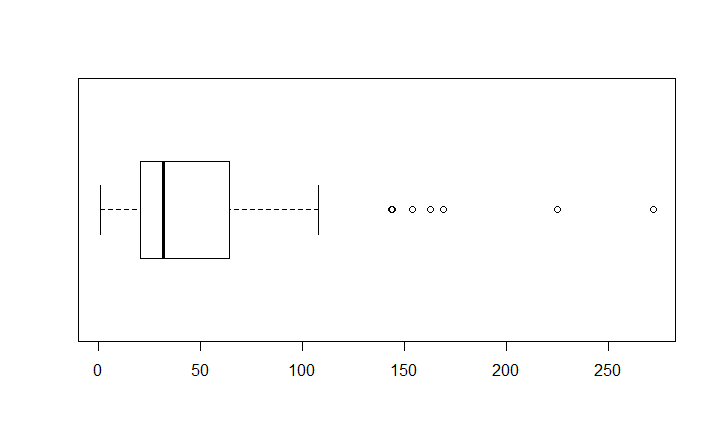
\includegraphics[scale=0.5]{boite.png}
\caption{Boîte à moustache}
\label{neutre}
\end{figure} 
\noindent La moyenne est à 48.89487 secondes. Le temps s'étend de 1.3s à 4min30s. Nous remarquons alors que des courbes elliptiques sont plus efficaces que d'autres. 
\begin{rem}
Des courbes elliptiques ont été construites pour qu'elles soient rapides pour certains algorithmes. 
En voici deux exemples.
\begin{enumerate}
\item  Curve25519 est une courbe elliptique très performante pour le protocole d'échange de clé de Diffie-Hellman. En particulier, c'est une courbe de Montgomery, qu'on verra au prochaine exemple.
\item Les courbes de Koblitz sont les courbes sur $\mathbb{F}_{2^k}$ de la forme suivante :
\begin{equation*}
y^2+xy=x^3+ax^2+1
\end{equation*}
Elles sont très appréciées pour les échanges de Bitcoin.
\end{enumerate}
\end{rem}

\noindent L'une des courbes elliptiques le plus rapide, pour l'algorithme de Lenstra, est la courbe de \textbf{Montgomery}. Elle est de la forme 
\begin{equation*}
By^2=x^3+Ax^2+x
\end{equation*}
On utilise alors une variante de l'algorithme Double-and-Add : \textbf{l'Echelle de Montgomery} \cite{ref17}. 
Cet algorithme est applicable à n'importe quelle courbe et peut être exécuté en coordonnées affines et projectives. Cependant, il est utile quand la courbe est de la forme de Montgomery en coordonnées projectives. Dans ce cas, tous les calculs peuvent être menées avec seulement les coordonnées $x$ et $z$. 
En effet, les formules de duplication dépendent de $x_{P-Q}$ et $z_{P-Q}$, et on peut faire en sorte que $P_{0}=(x_{0}::z_{0})=(x_{P-Q}::z_{P-Q})$. \\ \\
\fbox{
\begin{algorithm}[H]
\KwData{$P_{0}:=(x_{0}::z_{0})$ sur $C$ et $k:=(k_{s-1}k_{s-2}...k_{0})_{2}$}
 \KwResult{$kP_{0}$}
 $Q \leftarrow P_{0}; P \leftarrow 2P_{0}$ \\
 \For{$i$ from $s-2$ down to $0$}{
 \If{$k_{i}=1$} { $Q \leftarrow P+Q, P \leftarrow 2P$} 
 \If{$k_{i}=0$} { $P \leftarrow P+Q, Q \leftarrow 2Q$}
 }
 return $Q$
 \caption{Echelle de Montgomery}
\end{algorithm}}
\\
\begin{rem} 
\normalfont
La méthode de Lenstra  possède plusieurs avantages par rapport aux autres algorithmes de factorisation comme le crible algébrique et quadratique.
\begin{enumerate}
\item C'est la méthode la plus rapide si $n$ est divisible par un nombre premier qui est petit par rapport à $\sqrt{n}$.
Pour cette raison, elle peut être utilisé en combinaison avec d'autres algorithmes
\item Elle utilise très peu de mémoire par rapport à ses concurrentes.
\end{enumerate}

\end{rem}

Voici les différentes complexités des algorithmes présentés et de leurs concurrentes.
\begin{center}
\begin{tabular}{|l|c|}
  \hline
  Algirithmes & Compléxité  \\
  \hline
  Crible algébrique & $O(\text{exp}((\frac{64}{9}\log(n))^{\frac{1}{3}}\log(\log(n))^{\frac{2}{3}}))$  \\
  Crible quadratique & $O(\text{exp}(\sqrt{\log(n)\log(\log(n))})$  \\
  ECM & $O(\text{exp}(\sqrt{(1+\epsilon)\log(n)\log(\log(n))})$ \\
  p-1 Pollard & $O(k \log(k) \log^2(n))$ \\
  \hline
\end{tabular}
\end{center}
($\epsilon$ proche de $0$ pour $p$ grand et on rappelle que $k$ est une borne.) \\
L'auteur a tenté $M_{8}\times M_{9}$ avec l'algorithme $p-1$ Pollard et abandonna au bout de 3 heures.

\subsection{Clé d'échange de Diffie-Hellman}
\noindent L’échange de clé de Diffie-Hellman a été révélé en 1976 \cite{ref22}.
L’échange d’une clé secrète est important en cryptographie. Effectivement,  tout chiffrement d’une grande quantité de données ne peut se faire qu’avec du chiffrement à clé secrète, surtout si cet échange a lieu en temps réel, en raison de la lenteur des chiffrements à clé publique.
Il s’agit alors d’échanger entre deux interlocuteurs une clé secrète. 
Les clés d'échange de Diffie-Hellman sur les courbes elliptiques  sont très utilisés de nos jours. Elles proposent des clés plus courtes que celles du RSA et le niveau de sécurité est la même que des ses concurrentes.
En effet, une troisième personne doit résoudre ECDLP puiqu'il doit retouver $n_{A}$ de $n_{A}P$.
L'échange de Diffie-Hellman est sensible à l'attaque de l'homme du milieu. En effet, si une troisième personne intercepte les communications entre Alice et Bob alors elle peut se faire passer pour Bob ou Alice.
\begin{center}
\begin{tabular}{|c|c|} 
\hline

\multicolumn{1}{|c|}{Données publiques}  \\ 
 
\hline
$p$ premier, $C$ courbe elliptique sur $\mathbb{F}_{q}$ et un point $P$  \\
\hline
\end{tabular}
\end{center}

\begin{center}
\begin{tabular}{|c|c|} 
\hline

\multicolumn{1}{|c|}{Données Privées}  \\ 
 
\hline
Alice et Bob choisissent chacun un nombre entier. ($n_{A}$ pour Alice et $n_{B}$ pour Bob). \\ 
\hline
Alice calcule $Q_{A}=n_{A}P$ et envoie $Q_{A}$ à Bob.\\ 
Bob calcule $Q_{B}=n_{B}P$ et envoie $Q_{B}$ à Alice.  \\ \hline
Alice calcule $n_{A}Q_{B}$ \\
Bob calcule $n_{B}Q_{A}$ \\
\hline
La clé secrète commune est $n_{A}Q_{B}=n_{A}(n_{B}P)=n_{B}(n_{A}P)=n_{B}Q_{A}$. \\
\hline
\end{tabular}
\end{center}

\subsection{Algorithmes de comptage de points}

\noindent Actuellement, la pensée courante, introduite par Koblitz et Miller, est que pour les courbes elliptique sur les corps finis, la difficulté du logarithme discrète croît exponentiellement avec la taille du plus grand facteur du cardinal du groupe. Le théorème de Hasse nous renseigne sur un intervalle contenant le cardinal.
Un algorithme naïf pour le comptage des points est l'algorithme de
\textbf{Baby-step Giant-step} ou \textbf{algorithme de Shanks}. Le principe est de calculer des points dans deux listes jusqu'à leur "collision" i.e un point commun. 
\ \\ \\
La méthode est la suivante :
\begin{enumerate}
\item Procédons au \textit{baby-step} : calculer $P,2P,...,sP$ avec $s \approx p^{1/4}$.
\item Calculer $Q=(2s+1)P$ et $R=(p+1)P$.
\item Procédons au \textit{giant-step} : calculer $R,R \pm Q,R \pm 2Q,.., R \pm tQ$ avec \\ $t=\frac{2\sqrt{p}}{2s-1} \approx p^{1/4}$.
\item Par le théorème de Hasse, pour $i=0,\pm 1,\pm 2 ,..., \pm t$, $R \pm iQ$ est égal à un des points de la liste du \textit{baby-step}. Pour ce $i$, $R+iQ=jP$.
Alors $\#C(\mathbb{F}_{q})=p+1+(2s+1)i-j$.
\end{enumerate}

\noindent L'inconvénient est que la compléxité est  exponentielle.
Une percée majeure pour ce problème est l'\textbf{algorithme de Schoof} publié par René Schoof en 1985 \cite{ref18}.
C'est le premier algorithme à temps polynomial.
Son principe est basée sur la proposition suivante qu'on ne démontera pas.
\begin{prop}
Soit $\phi : C(\overline{\mathbb{F}_{q}}) \rightarrow C(\overline{\mathbb{F}_{q}})$ définie par  
\begin{equation*}
\phi((x,y))=(x^q,y^q)
\end{equation*}
l'homomorphisme de Frobenius où $\overline{\mathbb{F}_{q}}$ est la clôture algébrique de $\mathbb{F}_{q}$.
Définissons la trace de $\phi$ par  $tr(\phi)=q+1-\# C(\mathbb{F}_{q})$.
\begin{enumerate} 
\item $\phi^2 - (tr(\phi))\phi+q=0$ (Ce polynôme est appelé le polynôme caractéristique de Frobenius).
\item Pour les points $P=(X,Y)$ d'ordres $l$ finis, on a : 
\begin{equation*}
(X^{q^2}+Y^{q^2})+ [q \mod l](X,Y)=[tr(\phi) \mod l](X^q,Y^q)
\end{equation*}
\end{enumerate}
\end{prop}
\noindent L’algorithme consiste alors à calculer la partie gauche de l’équation  pour un point P d’ordre $l$ puis à calculer la partie droite jusqu'à que l'égalité soit vraie. On réitère et par le théorème des restes chinois, on peut trouver $tr(\phi)$. 
\begin{rem}
De nombreuses améliorations ont été réalisés dans les années 90 par Elkies et Atkin \cite{ref19}. L'algorithme est aujourd'hui nommé par \textbf{SEA}(Schoof-Elkies-Atkin). Il est implémenté comme un algorithme probabiliste (du type Las Vegas).
\end{rem}


\subsection{Tests de Primalité}
\noindent Les tests de primalité sont primordials pour la cryptographie.
L'idée de l'utilisation des courbes elliptiques pour des tests de primalités date de 1986 et a été promue par Shafi Goldwasser et Joe Kilian. L'usage des courbes elliptiques permettent des tests de primalité rapide et peuvent être implémentés.
L'algorithme le plus connu est celui de Goldwasser-Killian qui fut amélioré par Atkin et Morin \cite{ref19}.
L'algorithme de Goldwasser-Killian est basé sur ce théorème  \cite{ref23}.

\begin{theorem}[Goldwasser,Kilian] \label{gold}
Soient $n$ un entier premier avec 6, $C$ une courbe elliptique sur $\mathbb{Z}/n\mathbb{Z}$, $P$ un point de $C$ et $s,m$ deux entiers telles que $s|m$. \\
 Pour chaque $q$ premier divisant $s$, posons $(\frac{m}{q})P=(x_{q}:y_{q}:z_{q})$. 
Supposons que $mP=\mathcal{O}$ et $pgcd(z_{q},n)=1$ pour chaque $q$. \\
Alors il existe $p$ premier divisant $n$ tel que $\#C(\mathbb{F}_{p}) \equiv 0 [s]$.
\end{theorem}


\begin{cor}[Goldwasser,Kilian]
Soient $n$ un entier naturel et $C$ une courbe elliptique sur $\mathbb{Z}/n\mathbb{Z}$. Supposons qu'il existe $Q \in C(\mathbb{Z}/n\mathbb{Z})$ d'ordre $s$ avec \\
$s > (n^{1/4}+1)^2$. Alors
$n$ est premier. 
\end{cor}
\begin{preuve} 
\normalfont
Soit $p$ un diviseur de $n$. On a $\#C(\mathbb{Z}/p\mathbb{Z}) > (n^{1/4}+1)^2 $. D'après le théorème de Hasse,
$ \#C(\mathbb{Z}/p\mathbb{Z}) \leqslant (\sqrt{p}+1)^2$. D'où
\begin{equation*}
(\sqrt{p}+1)^2 > (n^{1/4}+1)^2.
\end{equation*}
Ainsi, tout diviseur $p$ de $n$ vérifie $p>\sqrt{n}$. Ainsi $n$ est premier. \qed
\end{preuve}
\noindent L'algorithme de Goldwasser-Kilian, pour un entier $p$, consiste à prouver que ce nombre est premier. 
On peut résumer l'algorithme ainsi :
\\
On veut tester la primalité de $n$.
\begin{enumerate}
\item Choisir une courbe elliptique sur $\mathbb{Z}/n\mathbb{Z}$ telle que $\#C(\mathbb{Z}/n\mathbb{Z})$ est de la forme $2q$ avec $q$ "premier probablement".
\item Si $(C,\#C(\mathbb{Z}/n\mathbb{Z}))$ satisfait les conditions du théorème \ref{gold} avec $s=\#C(\mathbb{Z}/n\mathbb{Z})$ alors $n$ est premier, sinon $n$ est composé.
\item La primalité de $q$ est faite de la même manière.
\end{enumerate}

\newpage
\section{Courbes elliptiques sur le corps des nombres complexes}

\noindent Tout au long de cette section IV, les courbes elliptiques sont définis sur le corps des nombres complexes $\mathbb{C}$.

\noindent Les courbes elliptiques sur $\mathbb{C}$ possèdent des propriétés intéressantes. Sa richesse provient des nombreux liens réalisés avec d'autres domaines dont l'analyse complexe et surtout l'arithmétique (avec les formes modulaires).
Plusieurs notions apparaissent dans cette théorie : les intégrales elliptiques, les fonctions elliptiques, le $j$-invariant et les formes modulaires. Dans la première partie, nous allons voir les correspondances entre les courbes elliptiques et les tores complexes par les fonctions elliptiques. Ensuite, nous utiliserons les fonctions modulaires pour classifier les courbes elliptiques. Nous allons finir ce mémoire par des courbes elliptiques particulières dites munies d'une multiplication complexe.

\subsection{Fonctions elliptiques}

\noindent Un sujet classique des courbes elliptiques est la théorie des fonctions 
elliptiques i.e  lesfonctions méromorphes sur $\mathbb{C}$. Historiquement, Niels Abel a découvert ces fonctions comme fonctions réciproques des intégrales elliptiques, le nom provenant du calcul de la longueur d'arc d'une ellipse.
Grâce à cette notion, nous pourrons voir que sur $\mathbb{C}$, une courbe elliptique est identifiée à un tore. 
Tout d'abord, définissons la notion de réseau et de fonction elliptique.
\begin{definition}
\begin{enumerate}
\item
Soit $\omega_{1},\omega_{2} \in \mathbb{C}$ tel que $\frac{\omega_{2}}{\omega_{1}} \not \in \mathbb{R}$. Un \textbf{réseau} $\Lambda$ du plan complexe est un 
sous-groupe abélien libre de rang 2. Il peut s'écrire
$\Lambda=\{\mathbb{Z}\omega_{1}+\mathbb{Z}\omega_{2} \} $.
\item
 Une \textbf{fonction elliptique}, pour un réseau $\Lambda$, est une fonction méromorphe $f(z)$ d'une variable complexe telle que
\begin{equation*}
\text{pour} \hspace{0.1cm} \text{tout} \hspace{0.1cm} \omega \in \Lambda, z \in \mathbb{C}  \hspace{1cm} f(z+\omega)=f(z).
\end{equation*}
On les appelle parfois \textbf{fonctions doublement périodiques}. On note $\mathbb{C}(\Lambda)$ l'ensemble de telles fonctions.
\item Un \textbf{parallélogramme fondamental} pour $\Lambda$ est l'ensemble
\begin{equation*}
D=\{a+t_{1}\omega_{1}+t_{2}\omega_{2} : 0 \leqslant t_{1},t_{2} <1 \}
\end{equation*}
où $a \in \mathbb{C}$, $\omega_{1},\omega_{2} \in \mathbb{C}$ tels que $\frac{\omega_{2}}{\omega_{1}} \not \in \mathbb{R}$.
\end{enumerate}
\end{definition}
\begin{figure}[!h]
\centering
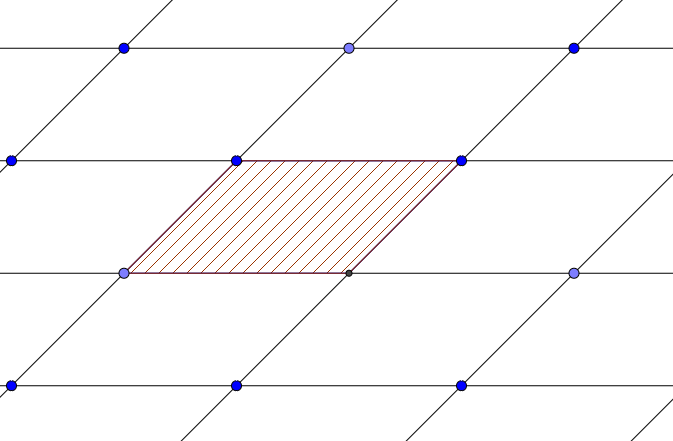
\includegraphics[scale=0.49]{test.png}
\caption{Un réseau avec un parallélogramme fondamental}
\label{neutre}
\end{figure}
\newpage
 \noindent Rappelons un théorème classique issu de l'analyse complexe. Voir \cite{ref29} pour une démonstration.

\begin{theorem}[Théorème de Liouville]\label{liou}
Une fonction holomorphe sur $\mathbb{C}$ et bornée est constante.
\end{theorem}
\noindent Nous pouvons maintenant démontrer le lemme suivant :
\begin{lem}[Liouville\footnote{Ce lemme est dû à Liouville alors que le théorème \ref{liou} est dû en réalité à Cauchy.}] \label{lemm1}
Une fonction elliptique qui n'a aucun pôle est constante.
\end{lem} 
\begin{proof}
Soient $f$ une fonction elliptique sur un réseau $\Lambda$ n'admettant aucun pôle et $D$  un parallélogramme fondamental. Comme $f$ n'admet aucun pôle, on a 
\begin{equation*}
\underset{z \in \mathbb{C}} \sup |f(z)|=\underset{z \in \overline{D}}\sup |f(z)|.
\end{equation*}
Sachant que $f$ est continue sur un compact $\overline{D}$ alors $|f(z)|$ est bornée sur $\overline{D}$ donc aussi sur $\mathbb{C}$. Par le théorème de Liouville, $f$ est constante.
\end{proof}


\noindent Par la suite, on note le résidu de $f$ au point $\omega$ Res($f$,$\omega$) et l'ordre de $f$ en $\omega$ est noté Ord($f$,$\omega$).


\begin{theorem}[\cite{ref2}] \label{theo2}
 Soient $f$ une fonction elliptique sur un réseau $\Lambda$ et $D$  un parallélogramme fondamental. Alors :
\begin{enumerate}
\item $\sum \limits_{\omega \in D} Res(f,\omega) = 0$.
\item $\sum \limits_{\omega \in D} Ord(f,\omega) = 0$.
\end{enumerate}
\end{theorem}

\begin{proof}
\begin{enumerate}
\item Posons $a,a+\omega_{1},a+\omega_{2}$ et $a+\omega_{1}+\omega_{2}$ les sommets de $D$. Par le théorème des résidus, nous obtenons 
\begin{align*}
\noindent \sum \limits_{\omega \in D} \text{Res}(f,\omega) & = 
\frac{1}{2\pi i} \int_{\partial D}^{} f(z) \, \mathrm{d}z 
 =  \frac{1}{2\pi i} (I_{1}+I_{2})
\end{align*}
où \begin{equation*}
I_{1}=\int_{a}^{a+\omega_{1}} f(z) \, \mathrm{d}z \hspace{0.1cm} +\int_{a+\omega_{2}}^{a} f(z) \, \mathrm{d}z 
\hspace{0.65cm}
I_{2}=
\int_{a+\omega_{1}}^{a+\omega_{1}+\omega_{2}} f(z) \, \mathrm{d}z \hspace{0.1cm}+ \int_{a+\omega_{1}+\omega_{2}}^{a+\omega_{2}} f(z) \, \mathrm{d}z.
\end{equation*}
Par changement de variables, il est clair que
\begin{equation*}
I_{2}=\int_{a}^{a+\omega_{2}} f(z+\omega_{1}) \, \mathrm{d}z+\int_{a+\omega_{1}}^{a} f(z+\omega_{2}) \, \mathrm{d}z
\end{equation*}
En réorganisant les termes et comme $f$ est doublement périodique, nous obtenons
\begin{align*}
  \sum \limits_{\omega \in D} \text{Res}(f,\omega) & =  \frac{1}{2\pi i}\Big(\int_{a}^{a+\omega_{1}} f(z)-f(z+\omega_{2}) \, \mathrm{d}z -\int_{a}^{a+\omega_{2}} f(z)-f(z+\omega_{1}) \, \mathrm{d}z \Big) \\
   &=0.
\end{align*}
\item Comme $f'$ est périodique par la périodicité de $f$, on peut appliquer 1) au quotient  
$f'/f \in \mathbb{C}(\Lambda)$. Nous avons alors
\begin{equation*}
\sum \limits_{\omega \in D} \text{Ord}(f,\omega)=\frac{1}{2\pi i}\int_{\partial D}^{} \frac{f'(z)}{f(z)} \, \mathrm{d}z=0.
\end{equation*}
\end{enumerate}
\end{proof}

\noindent L'ordre d'une fonction elliptique est la somme des ordres des pôles de tout parallélogramme fondamental. Une conséquence immédiate du théorème est alors:

\begin{cor}[\cite{ref2}]
Une fonction elliptique non-constante est d'ordre supérieure à 2.
\end{cor}

\begin{proof}
Supposons, par l'absurde, que $f$ est d'ordre 1. Un de ses résidus doit être non nul, ce qui contredit le théorème précédent.
\end{proof}

\noindent Pour illustrer ces notions, étudions une classe importante des fonctions elliptiques : la fonction $\wp$ de Weierstrass.

\begin{definition}
La fonction $\wp$ de Weierstrass est définie par :
\begin{equation*}
\wp(z)=\frac{1}{z^2}+\sum \limits_{\omega \in \Lambda'} \frac{1}{(z-\omega)^2}-\frac{1}{\omega^2}
\end{equation*}
où $\Lambda'=\Lambda \hspace{0.1cm} \backslash \hspace{0.1cm} \{0\}$.
\end{definition}

\noindent La convergence est bien définie par le théorème suivant.

\begin{theorem}[\cite{ref2}] \label{theo3}
Soit $\Lambda$ un réseau.
\begin{enumerate}
\item La série de la fonction $\wp$  converge absolument et uniformément sur chaque compact de $\mathbb{C} \hspace{0.1cm} \backslash \hspace{0.1cm} \Lambda$. 
La fonction est alors méromorphe sur $\mathbb{C}$.
\item La fonction $\wp$  est une fonction elliptique paire.
\end{enumerate}
\end{theorem}
\begin{proof}
Tout d'abord, démontrons le lemme suivant.

\begin{lem}[\cite{ref2}]\label{eisen}
La série $G_{2k}$ définie par 
\begin{equation*}
G_{2k}(\Lambda)=\sum \limits_{\omega \in \Lambda'} \frac{1}{\omega^{2k}}
\end{equation*}
où $\Lambda'=\Lambda \hspace{0.1cm} \backslash \hspace{0.1cm} \{0\}$, converge absolument pour $k>1$. La série $G_{2k}$ est appelé la série d'Eisenstein de poids $2k$.
\end{lem}


\begin{proof}
Comme $\Lambda$ est discret, il existe une constante     $c$ tel que pour tout entier naturel $n$ non nul
\begin{equation*}
\#\{\omega \in \Lambda : n \leqslant |\omega| < n+1\} <cn.
\end{equation*}
Par conséquent,
\begin{equation*}
\sum \limits_{\substack{ \omega\in \Lambda \\ |\omega|\geqslant 1}} \frac{1}{|\omega|^{2k}} \leqslant \sum \limits_{n=1}^\infty \frac{\#\{\omega \in \Lambda : n \leqslant |\omega| < n+1\}}{n^{2k}} < \sum \limits_{n=1}^\infty \frac{c}{n^{2k-1}}<\infty.
\end{equation*}
\end{proof}
\noindent On revient à la preuve du théorème \ref{theo3}.
\begin{enumerate}
\item
Montrons que la série converge uniformément sur les disques $|z| \leqslant R$. Sachant que le réseau est discret, l'intersection avec les disques est finie et on a $\omega \geqslant 2R$ pour tout $\omega$ sauf un nombre fini.
Pour $\omega \geqslant 2R$ et $z$ dans le disque de rayon $R$, on a 
\begin{equation*}
\Bigg|\frac{1}{(z-\omega)^2}-\frac{1}{\omega^2}\Bigg|=\Bigg| \frac{|z| |2-\frac{z}{\omega}|}{|\omega^3| |1-\frac{z}{\omega}|} \Bigg|.
\end{equation*}
Or $|z| \leqslant R, |2-\frac{z}{\omega}|\leqslant \frac{5}{2}$ et $|1-\frac{z}{\omega}| \geqslant \frac{1}{2}$ d'où 
\begin{equation*}
\Bigg|\frac{1}{(z-\omega)^2}-\frac{1}{\omega^2}\Bigg| \leqslant \frac{10R}{|\omega|^3}.
\end{equation*}
Par le lemme précédent, nous avons bien le résultat souhaité.
\item En remplaçant $\omega$ par $-\omega$, il est clair que $\wp(-z)=\wp(z)$.
Comme la série de $\wp$ converge uniformément, la dérivée est bien définie et nous pouvons dériver terme à terme. Nous obtenons
\begin{equation} \label{equa}
\wp'(z)=-2 \sum \limits_{\omega \in \Lambda} \frac{1}{(z-\omega)^3}.
\end{equation}
Il est aussi clair que $\wp'$ est une fonction elliptique. \\
En intégrant (\ref{equa}), on a
\begin{equation*}
\wp(z+\omega)-\wp(z)=c(\omega)
\end{equation*}
pour tout $z \in \mathbb{C} \backslash \Lambda$, où $c(\omega) \in \mathbb{C}$ est indépendant de $z$.
En posant $z=\omega/2$, l'équation devient 
\begin{equation*}
\wp\Big(\frac{\omega}{2}\Big)-\wp\Big(\frac{-\omega}{2}\Big)=c(\omega).
\end{equation*}
Comme la fonction $\wp$ est paire, $c(\omega)=0$, ce qui conclut la démonstration.
\end{enumerate}
\end{proof}
\noindent Le prochain théorème est crucial, il nous dit que toute fonction elliptique peut être exprimée par la fonction $\wp$ de Weierstrass et ainsi on peut se focaliser sur $\wp$.

\begin{theorem}[\cite{ref2}] \label{theo6}
Soit $\Lambda$ un réseau de $\mathbb{C}$. Toute fonction elliptique est une fraction rationnelle de $\wp$ et $\wp'$. Autrement dit, $\mathbb{C}(\Lambda)=\mathbb{C}(\wp(z),\wp'(z))$.
\end{theorem}



\begin{proof}
Tout d'abord, montrons que toute fonction elliptique paire est une fraction rationnelle de $\wp$. Pour cela, nous utilisons le lemme suivant :
\begin{lem}
\begin{enumerate}
\item Soient $f$ une fonction paire sur $\mathbb{C}(\Lambda)\backslash \mathbb{C}$ et $a \in \mathbb{C}$ tel que \\$2a \in \Lambda$. Alors $\text{Ord}(f,a)$ est un entier pair.
\item 
Pour $a \in \mathbb{C} \backslash \Lambda$, la fonction $h_a : z \mapsto \wp(z) - \wp(a)$ possède un zéro aux points $\pm a$ si $2a \not \in \Lambda$, un zéro d'ordre 2 si $2a \in \Lambda$.
\end{enumerate}
\end{lem}

\begin{proof}
\begin{enumerate}
\item
Le développement de Taylor de $f$ en $a$ est
\begin{equation*}
f(z)=c_m(z-a)^m+c_{m+1}(z-a)^{m+1}+... \hspace{1cm}c_m \neq 0.
\end{equation*}
La périodicité de $f$ nous donne
\begin{equation*}
f(z)=f(-z+2a)=(-1)^mc_m(z-a)^m+...
\end{equation*}
d'où $m=\text{Ord}(f,a)$ est pair.
\item Comme $\wp$ (et donc $h_a$) possède un unique pôle, d'après le théorème \ref{theo2}, la somme des ordres des zéros de $h_a$ est égal à l'ordre du pôle i.e 2. Donc si $2a \not \in \Lambda$, $a$ et $-a$ sont deux zéros  de $h_a$. D'après 1), si $2a \in \Lambda$, $a$ est d'ordre exactement 2.
\end{enumerate}
\end{proof}
Soient $f$ une fonction elliptique paire et $a_1,...,a_s$ les points où $\text{Ord}(f,a_i) \neq 0$ pour tout $i\in \{1,...,s\}$. Posons $m'_i=\text{Ord}(f,a_i)$ si $2a_i \not \in \Lambda$, $m'_i=\text{Ord}(f,a_i)/2$ sinon. Posons 
\begin{equation*}
g(z)=f(z) \prod \limits_{i=1}^s(\wp(z)-\wp(a_i))^{-m'_i}
\end{equation*}
Par le lemme précédent, $g$ ne possède des zéros ou pôles que sur $\Lambda$. Par le lemme \ref{lemm1}, $g$ est constante donc $f$ est une fonction rationnelle de $\wp$. \\
Maintenant, nous supposons que $f$ est une fonction elliptique quelconque. On peut écrire $f$ sous la forme
\begin{equation*}
f(z)=\frac{f(z)+f(-z)}{2}+\frac{f(z)-f(-z)}{2\wp'(z)}\wp'(z).
\end{equation*}
La fonction $f$ est alors une combinaison de 1 et $\wp'$ dont les coefficients sont des fonctions elliptiques paires. On conclut alors que $f$ est rationnelle de $\wp$ et $\wp'$.

\end{proof}


\noindent Le lien entre les courbes elliptiques et les fonctions elliptiques est réalisé par le fait que $\wp$ est solution d'une équation différentielle. Cette démonstration est basée sur sa série de Laurent.



\begin{theorem} [\cite{ref2}] \label{theo4}
\begin{enumerate}
\item La série de Laurent de $\wp(z)$ autour de $z=0$ est donnée par 
\begin{equation*}
\wp(z)=\frac{1}{z^2}+ \sum \limits_{k=1}^{\infty} (2k+1)G_{2k+2}z^{2k}
\end{equation*}
où $G_{2k}$ est la série d'Eisenstein définie dans le lemme \ref{eisen}.
\item $\forall z \in \mathbb{C} \backslash \Lambda$, 
\begin{equation*}
\wp'(z)^2=4\wp(z)^3-60G_{4}\wp(z)-140G_{6}.
\end{equation*}
\end{enumerate}
\end{theorem}

\begin{proof}
\begin{enumerate}
\item Pour $|z| < |\omega|$, on a
\begin{equation*}
 \frac{1}{(z-\omega)^2}-\frac{1}{\omega^2}=\frac{1}{\omega^2} \Bigg[ \frac{1}{(1-\frac{z}{\omega})^2}-1 \Bigg]= \sum \limits_{n=1}^{\infty} \frac{(n+1)z^n}{\omega^{n+2}}
\end{equation*}
d'où
\begin{equation*}
\wp(z)=\frac{1}{z^2}+\sum \limits_{\omega \in \Lambda'}
\sum \limits_{n=1}^{\infty} \frac{(n+1)z^n}{\omega^{n+2}}.
\end{equation*}
Comme la série converge absolument et que $G_{2k+1}=0$ pour $k>1$, on a bien le résultat.
\item Calculons les premiers termes des séries de Laurent de $\wp(z),\wp'(z)^2$ et $\wp(z)^3$.
\begin{align*}
\wp(z) &= \frac{1}{z^2}+3G_{4}z^2+... \\
\wp'(z)^2 &= \frac{4}{z^6}-\frac{24G_{4}}{z^2}-80G_{6}+... \\
\wp(z)^3 &=\frac{1}{z^6}+\frac{9G_{4}}{z^2}+15G_{6}+...
\end{align*}
Posons la fonction
\begin{equation*}
f(z)=\wp'(z)^2-4\wp(z)^3+60G_{4}\wp(z)+140G_{6}=\frac{(60G_{4})^2}{20}z^2+\frac{(60G_{4})(140G_{6})}{28}z^4+...
\end{equation*}
La fonction $f$ est holomorphe autour de $z=0$ et satisfait $f(0)=0$. Par le théorème \ref{theo3}, $f$ est une fonction elliptique sans pôle. Par le lemme \ref{lemm1} et comme $f(0)=0$ alors $f$ est la fonction nulle d'où le résultat.
\end{enumerate}
\end{proof}


\noindent 
On rappelle qu'une courbe elliptique peut être réduit à une forme de Weierstrass $y^2=x^3+ax+b$. Par le changement de variable $y \mapsto \frac{1}{2} y$, on peut se ramener à 
\begin{equation*}
y^2=4x^3-g_2x-g_3
\end{equation*}
Maintenant, on peut montrer la correspondance entre les tores complexes et les courbes elliptiques.

\begin{theorem}[\cite{ref2}] \label{theo5}
Soient $\Lambda$ un réseau, $\wp$ la fonction de Weierstrass et $C$ une courbe elliptique de la forme
\begin{equation*}
y^2=4x^3-g_{2}x-g_{3}.
\end{equation*}
L'application 
\begin{align*}
\Psi : \mathbb{C} / \Lambda \rightarrow C \subset \mathbb{P}^2(\mathbb{C})   \hspace{1cm} z &\mapsto (\wp(z):\wp'(z):1) \\ 0&\mapsto (0:1:0)
\end{align*}
est une bijection entre le tore complexe $\mathbb{C}/ \Lambda$ et la courbe elliptique $C$.
\end{theorem}

\begin{proof}
Montrons, tout d'abord, que $\Psi$ est surjective. 
Par le théorème \ref{theo4}, Im$(\Psi) \subset C$.
Soit $P=(x,y)\in C$.
Alors $\wp(z)-x$ est une fonction elliptique non constante donc d'après le lemme \ref{lemm1}, elle possède un pôle, disons $z=a$.
Il s'ensuit que $\wp'(a)^2=y^2$. Quitte à remplacer $a$ par $-a$ au besoin, nous avons $\Psi'(a)=y$. D'où $\psi(a)=(x,y)$, ce qui démontre la surjectivité. \\
Supposons maintenant que $\Psi(z_{1})=\Psi(z_{2})$. Nous distinguons deux cas : 
supposons que $2z_{1} \notin \Lambda$. Alors la fonction $\wp(z)-\wp(z_{1})$ est d'ordre 2 et dont les zéros sont $z_{1},-z_{1}$ et $z_{2}$. Par conséquent, 
\begin{equation*}
z_{2} \equiv \pm z_{1} \mod \Lambda
\hspace{1cm} \text{et} \hspace{1cm}
\wp'(z_{1})=\wp'(z_{2})=\wp'(\pm z_{1})=\pm \wp'(z_{1}).
\end{equation*}
Ainsi, $z_{2} \equiv z_{1} \mod \Lambda$. \\
De manière similaire, si $2z_{1} \notin \Lambda$, $\wp(z)-\wp(z_{1})$ a un zéro d'ordre 2 en $z_{1}$ et s'annule en $z_{2}$. La conclusion est alors la même : $z_{2} \equiv z_{1} \mod \Lambda$. Ainsi $\Psi$ est injective, et cela conclut la preuve.
\end{proof}

\begin{theorem}[\cite{ref2}]
L'application $\Psi$, définie dans le théorème \ref{theo5},
\begin{align*}
\Psi : \mathbb{C} / \Lambda \rightarrow C \subset \mathbb{P}^2(\mathbb{C})   \hspace{1cm} z &\mapsto (\wp(z):\wp'(z):1)) \\ 0&\mapsto (0:1:0)
\end{align*}
est un biholomorphisme.
\end{theorem}
\noindent 
Nous ne démontrerons pas ce résultat, la preuve fait intervenir le groupe d'homologie $H_{1}(C,\mathbb{Z})$. \\

\begin{rem}\label{rem1}
\normalfont Le théorème \ref{theo5} montre qu'à tout réseau $\Lambda$ de $\mathbb{C}$, on peut associer une courbe elliptique. Le théorème d'uniformisation (que nous verrons dans la section IV.2) est la réciproque. Il nous dit que toute courbe elliptique sur $\mathbb{C}$ est paramétrée par les fonctions elliptiques.
\end{rem}

\noindent Avant de poursuivre, nous allons définir la notion d'isogénie. Les isogénies seront notamment utilisées dans la section 'Multiplication complexe'.

\begin{definition}
\begin{enumerate}
\item
Soient $C_{1},C_{2}$ deux courbes elliptiques.
Une \textbf{isogénie} de $C_{1}$ dans $C_{2}$ est un morphisme de groupe $\phi : C_{1} \rightarrow C_{2}$ préservant l'élément neutre.
\item L'\textbf{anneau des endomorphismes} d'une courbe elliptique $C$ est l'ensemble End($C)=\{ \phi :C \rightarrow C : \phi$ isogénie $\} \cup \{0\}$.
\end{enumerate}
\end{definition}

\begin{rem}
Généralement, on définit une isogénie comme un morphisme de groupe algébrique qui est surjectif et qui a un noyau fini.
\end{rem}

\begin{ex}[\cite{ref}]
\begin{enumerate}
\item \normalfont  Les applications définies dans la sous-lemme \ref{prop1} sont des isogénies.
\begin{align*}
\phi : C_{1} &\rightarrow C_{2}  \\
(x,y) &\rightarrow \Big(\frac{y^2}{x^2},\frac{y(b-x^2)}{x^2} \Big) 
\end{align*}
La preuve de Mordell-Weil se fait avec des isogénies.
\item
Dans la section I.3, nous avons vu l'application
\begin{align*}
[n] : C &\rightarrow C \\
P &\mapsto nP
\end{align*}
où $n \in \mathbb{Z}$. Cette application est une isogénie. 
\end{enumerate}
\end{ex}
\noindent Pour finir cette partie, on veut montrer une correspondance entre les isogénies, les fonctions holomorphes et les réseaux homothétiques (i.e qui différent d'un élément de $\mathbb{C}^*$, voir \ref{cor2}).
\noindent Soient $\Lambda_{1},\Lambda_{2}$ deux réseaux de $\mathbb{C}$. On peut définir une fonction holomorphe, entre deux tores complexes, $\phi :\mathbb{C}/\Lambda_{1} \rightarrow \mathbb{C}/\Lambda_{2}$ par le diagramme suivant : 
\begin{equation*}
\xymatrix{
    \mathbb{C} \ar[r]^f \ar[d] & \mathbb{C} \ar[d] \\
    \mathbb{C}/\Lambda_{1} \ar[r]_\phi & \mathbb{C}/\Lambda_{2}
  }
\end{equation*}
Ce diagramme commute car $\mathbb{C}$ est simplement connexe.





\begin{theorem}[\cite{ref2}] \label{theo7}
Soient $\Lambda_{1},\Lambda_{2}$ deux réseaux de $\mathbb{C}$. Posons $\mathcal{H}$ l'ensemble des fonctions holomorphes $\phi :\mathbb{C}/\Lambda_{1} \rightarrow \mathbb{C}/\Lambda_{2}$ avec $\phi(0)=0$.
\begin{enumerate}
\item Soit l'application $\phi_{\alpha}$ : 
\begin{equation*}
\phi_{\alpha} : \mathbb{C}/\Lambda_{1} \rightarrow \mathbb{C}/\Lambda_{2} \hspace{1.5cm} \phi_{\alpha}(z)=\alpha z \mod \Lambda_{2}.
\end{equation*}
L'application
\begin{align*}
\{\alpha \in \mathbb{C} :\alpha \Lambda_{1} \subset \Lambda_{2} \} &\rightarrow \mathcal{H} \\
\alpha &\mapsto \phi_{\alpha}
\end{align*}
est une bijection.
\item Soient $C_{1},C_{2}$ deux courbes elliptiques correspondant aux réseaux $\Lambda_{1},\Lambda_{2}$.
Il existe une bijection 
\begin{equation*}
\psi : \{ \phi : C_{1} \rightarrow C_{2} : \phi \hspace{0.2cm} \text{isogénie} \} \rightarrow \mathcal{H}.
\end{equation*}
\end{enumerate}
\end{theorem}

\begin{proof}
\begin{enumerate}
\item
Supposons que $\phi_{\alpha}=\phi_{\beta}$ alors
\begin{equation*}
 \forall z \in \mathbb{C}, \hspace{1cm} \alpha z \equiv \beta z \mod \Lambda_{2}.
\end{equation*}
Par conséquent, l'application $z \mapsto (\alpha-\beta)z$ envoie $\mathbb{C}$ sur $\Lambda_{2}$. Comme $\Lambda_{2}$ est discret, cette application est constante d'où $\alpha=\beta$, l'application est alors injective. \\
Soit $\phi \in \mathcal{H}$.
On peut se ramener à une fonction holomorphe $f$ par le diagramme suivant
\begin{equation*}
\xymatrix{
    \mathbb{C} \ar[r]^f \ar[d] & \mathbb{C} \ar[d] \\
    \mathbb{C}/\Lambda_{1} \ar[r]_\phi & \mathbb{C}/\Lambda_{2}
  }
\end{equation*}
Ce diagramme commute car $\mathbb{C}$ est simplement connexe.
Ainsi 
\begin{equation*}
 \forall \omega \in \Lambda_{1}, \forall z \in \mathbb{C}, \hspace{1cm} f(z+\omega) \equiv f(z) \mod \Lambda_{2}.
\end{equation*}
Comme $\Lambda_{2}$ est discret, la quantité $f(z+\omega)-f(\omega)$ est indépendante de $z$. En dérivant,
\begin{equation*}
\forall \omega \in \Lambda_{1}, \forall z \in \mathbb{C}, \hspace{1cm} f'(z+\omega) = f'(z)
\end{equation*}
,on trouve alors que $f'(z)$ est une fonction elliptique. Par le lemme \ref{lemm1}, $f'(z)$ est constante d'où $f(z)$ est un polynôme en $z$ de degré 1. Comme $f(0)=0$, $f(z)$ est de la forme $\alpha z$. Ainsi $f(\Lambda_{1})=\alpha\Lambda_{1} \subset \Lambda_{2}$ d'où $\phi=\phi_{\alpha}$, ce qui conclut la première partie.

\item Par définition, une isogénie est un morphisme, l'image par $\psi$ est alors une fonction holomorphe entre les deux tores. L'application $\psi$ est alors bien définie et est clairement injective. \\
Pour la surjectivité, nous utilisons la correspondance vue en 1., en considérant l'application $\phi_{\alpha}$ avec $\alpha \in \mathbb{C}^*$ tel que $\alpha \Lambda_{1} \subset \Lambda_{2}$.
Par le théorème \ref{theo5}, on peut définir l'application suivante
\begin{align*}
C_{1} &\rightarrow C_{2} \\
(\wp(z,\Lambda_{1}):\wp'(z,\Lambda_{1}):1) &\mapsto (\wp(\alpha z,\Lambda_{2}):\wp'(\alpha z,\Lambda_{2}):1)
\end{align*}
où $\wp(z,\Lambda)$ correspond à la fonction de Weierstrass associée à $\Lambda$. En utilisant le théorème \ref{theo6}, si $\wp(\alpha z,\Lambda_{2})$ et $\wp'(\alpha z,\Lambda_{2})$ sont des fractions rationnelles en $\wp(\alpha z,\Lambda_{1})$ et $\wp'(\alpha z,\Lambda_{1})$ alors le théorème est démontré. \\
Comme $\alpha \Lambda_{1} \subset \Lambda_{2}$, nous avons, pour tout $\omega_{1} \in \Lambda_{1}$,
\begin{equation*}
\wp(\alpha(z+\omega),\Lambda_{2})=\wp(\alpha z+\alpha \omega,\Lambda_{2})=\wp(\alpha z,\Lambda_{2}).
\end{equation*}
Il en est de même pour $\wp'(\alpha z,\Lambda_{2})$.
Ainsi $\wp(\alpha z,\Lambda_{2}) \in \mathbb{C}(\Lambda_{1})$ et $\wp'(\alpha z,\Lambda_{2}) \in \mathbb{C}(\Lambda_{1})$ et le théorème est démontré.
\end{enumerate} 
\end{proof}



\begin{cor}[\cite{ref2}] \label{cor2}
Soient $C_{1}$ et $C_{2}$ deux courbes elliptiques de réseaux $\Lambda_{1},\Lambda_{2}$ respectivement. Les courbes $C_{1}$ et $C_{2}$ sont isomorphes si et seulement si il existe $\alpha \in \mathbb{C}^*$ tel que
$\Lambda_{1}=\alpha \Lambda_{2}$ (dans ce cas, on dit que $\Lambda_1$ et $\Lambda_2$ sont homothétiques).
\end{cor}

\noindent La preuve est admise.






















\begin{rem} [\cite{ref25}]
\normalfont
\noindent Posons $\wp(z)=w$, nous écrivons l'équation sous la forme
\begin{equation*}
\frac{dz}{dw}=\frac{1}{\sqrt{4w^3-4g_{2}-g_{3}}}
\end{equation*}
d'où nous concluons que $\wp(z)$ est la fonction inverse de l'intégrale 
\begin{equation*}
z-z_{0}=\int \limits_{\wp(z_{0})}^{w} \frac{dw}{\sqrt{4w^3-4g_{2}-g_{3}}}.
\end{equation*}
En faisant tendre $z_{0}$ vers $0$, nous obtenons l'intégrale elliptique sous forme de Weierstrass
\begin{equation*}
z=\int \limits_{\infty}^{w} \frac{dw}{\sqrt{4w^3-4g_{2}-g_{3}}}
\end{equation*}
dont l'inverse est la fonction $\wp$. \\
Historiquement, la notion de fonction elliptique provient des études sur les intégrales elliptiques et nous venons de voir ce lien. Le nom "elliptique" vient du fait que le calcul de longueur d'arc d'une ellipse donne une intégrale qui est de la forme vue précédemment.
\end{rem}


\subsection{Groupe modulaire}
\noindent Rappelons que le groupe $\text{SL}_{2}(\mathbb{Z})$ est défini par
\begin{equation*}
\text{SL}_{2}(\mathbb{Z})=\Big\{\begin{pmatrix} 
a & b \\
c & d 
\end{pmatrix} : a,b,c,d \in \mathbb{Z} \hspace{0.2cm} \text{et}
\hspace{0.2cm} ad-bc=1 \Big\}.
\end{equation*}
et on appelle \textbf{groupe modulaire} le groupe $\text{PSL}_{2}(\mathbb{Z})=\text{SL}_{2}(\mathbb{Z})/\{\pm \text{Id}_2\}$.
\\
\noindent Comme nous travaillons sur $\Lambda=\mathbb{Z}\omega_{1}+\mathbb{Z}\omega_{2}$ à homothétie près, on peut normaliser la base du réseau
\begin{equation*}
\frac{1}{\omega_{2}}\Lambda=\mathbb{Z}\frac{\omega_{1}}{\omega_{2}}+\mathbb{Z}.
\end{equation*}
On peut alors choisir $\omega_1,\omega_2 \in \mathbb{C}$ tel que $\Im(\omega_{1}/\omega_{2})>0$, ce qui nous suggère de travailler sur le demi-plan supérieur $\mathbb{H}=\{\tau \in \mathbb{C} : \Im(\tau)>0\}$ de $\mathbb{C}$. Le but de cette section est démontrer que pour $\tau, \tau' \in \mathbb{H}$, $C_\tau \cong \mathbb{C} /(\mathbb{Z}+\tau\mathbb{Z})$ et $C_{\tau'} \cong \mathbb{C} /(\mathbb{Z}+\tau'\mathbb{Z})$ sont isomorphes si et seulement si il existe
$ \begin{pmatrix} 
a & b \\
c & d 
\end{pmatrix} \in \text{SL}_{2}(\mathbb{Z})$ tel que $\tau'=\frac{a\tau+b}{c\tau+d}$.
\noindent On peut résumer cette section IV.2 de ce mémoire par le schéma suivant :
\begin{align*}
\mathcal{E}\mathscr{R}\mathscr{R}_\mathbb{C} &\xleftarrow{\makebox[1.4cm]{\ref{theo10}}} \mathscr{R}/\mathbb{C}^* \xleftarrow{\makebox[1cm]{\ref{theo10}}} \mathbb{H} /\text{SL}_{2}(\mathbb{Z}) \xrightarrow{\makebox[1cm]{\ref{lem8}}}  \mathbb{C} \\
\{C_\Lambda\} &\xleftarrow{\makebox[1cm]{}} \{\Lambda\}=\{\Lambda_\tau \} \xleftarrow{\makebox[0.5cm]{}}\hspace{0.3cm} \tau \hspace{0.6cm} \xrightarrow{\makebox[1.1cm]{}} j(\tau)
\end{align*}
où $\mathcal{E}\mathscr{R}\mathscr{R}_\mathbb{C}$ est l'ensemble des classes d'isomorphisme des courbes elliptiques et \\
$\Lambda_\tau=\mathbb{Z}+\tau\mathbb{Z}$.
\\
Pour démontrer cela, on va décrire l'action de groupe de $\text{SL}_2(\mathbb{Z})$ sur $\mathbb{H}$ (qui sera définie dans la proposition \ref{modul}) et on va  utiliser les fonctions modulaires pour démontrer le théorème d'uniformisation vu dans la remarque \ref{rem1}.


\begin{definition}
Soient $G$ un groupe et $X$ un ensemble sur lequel $G$ agit. On note $g.x$ l'image de $x \in X$ par l'action de l'élément $g \in G$. Un sous-ensemble $Y$ de $X$ est un \textbf{domaine fondamental} si : 
\begin{enumerate}
\item $\bigcup\limits_{g \in G} g.Y=X$.
\item $\forall g,g' \in G$ tels que $g \neq g'$, $g.Y \cap g'.Y = \emptyset$.
\end{enumerate}
Le domaine fondamental contient alors exactement un point par orbite du groupe.
\end{definition}

\begin{prop}[\cite{ref26}] \label{modul}
Avec les notations ci-dessus, on a :
\begin{enumerate}
\item Le groupe $SL_{2}(\mathbb{Z})$ agit sur $\mathbb{H}$ par
\begin{equation*}
\forall \gamma=\begin{pmatrix} 
a & b \\
c & d 
\end{pmatrix} \in SL_{2}(\mathbb{Z}), \forall \tau \in \mathbb{H}, \hspace{0.8cm}
\gamma.\tau=\frac{a\tau+b}{c\tau+d}.
\end{equation*}
Le groupe modulaire $PSL_{2}(\mathbb{Z})$ agit de la même manière sur $\mathbb{H}$. Le lemme \ref{leme1} montre que l'action du groupe modulaire sur $\mathbb{H}$ est fidèle.
\item 
Posons $\mathcal{F}'=\{\tau \in \mathbb{H} : |\Re(\tau)| \leqslant \frac{1}{2} \hspace{0.2cm} et \hspace{0.2cm} |\tau | \geqslant 1 \}$.
La région $\mathcal{F}$ de $\mathbb{H}$ définie par
\begin{equation*}
\mathcal{F}=\mathcal{F}' \hspace{0.1cm} \backslash \Big(\{\tau \in \mathcal{F} : \Re(\tau)=\frac{1}{2} \} \cup \{\tau \in \mathcal{F} : (|\tau|=1 \hspace{0.2cm} et \hspace{0.2cm} \Re(\tau)>0) \}\Big)
\end{equation*}
est un domaine fondamental pour l'action de groupe de $SL_{2}(\mathbb{Z})$ sur $\mathbb{H}$.
\item Le groupe modulaire $PSL_{2}(\mathbb{Z})$ est engendré par $S$ et $T$ où $S=\begin{pmatrix} 
0 & -1 \\
1 & 0 
\end{pmatrix}
$
et $T=\begin{pmatrix} 
1 & 1 \\
0 & 1 
\end{pmatrix}
$, ce qui équivaut à $S.\tau=-1/\tau$, $T.\tau =\tau+1$.
\end{enumerate}
\end{prop}

\begin{figure}[!h]
\centering
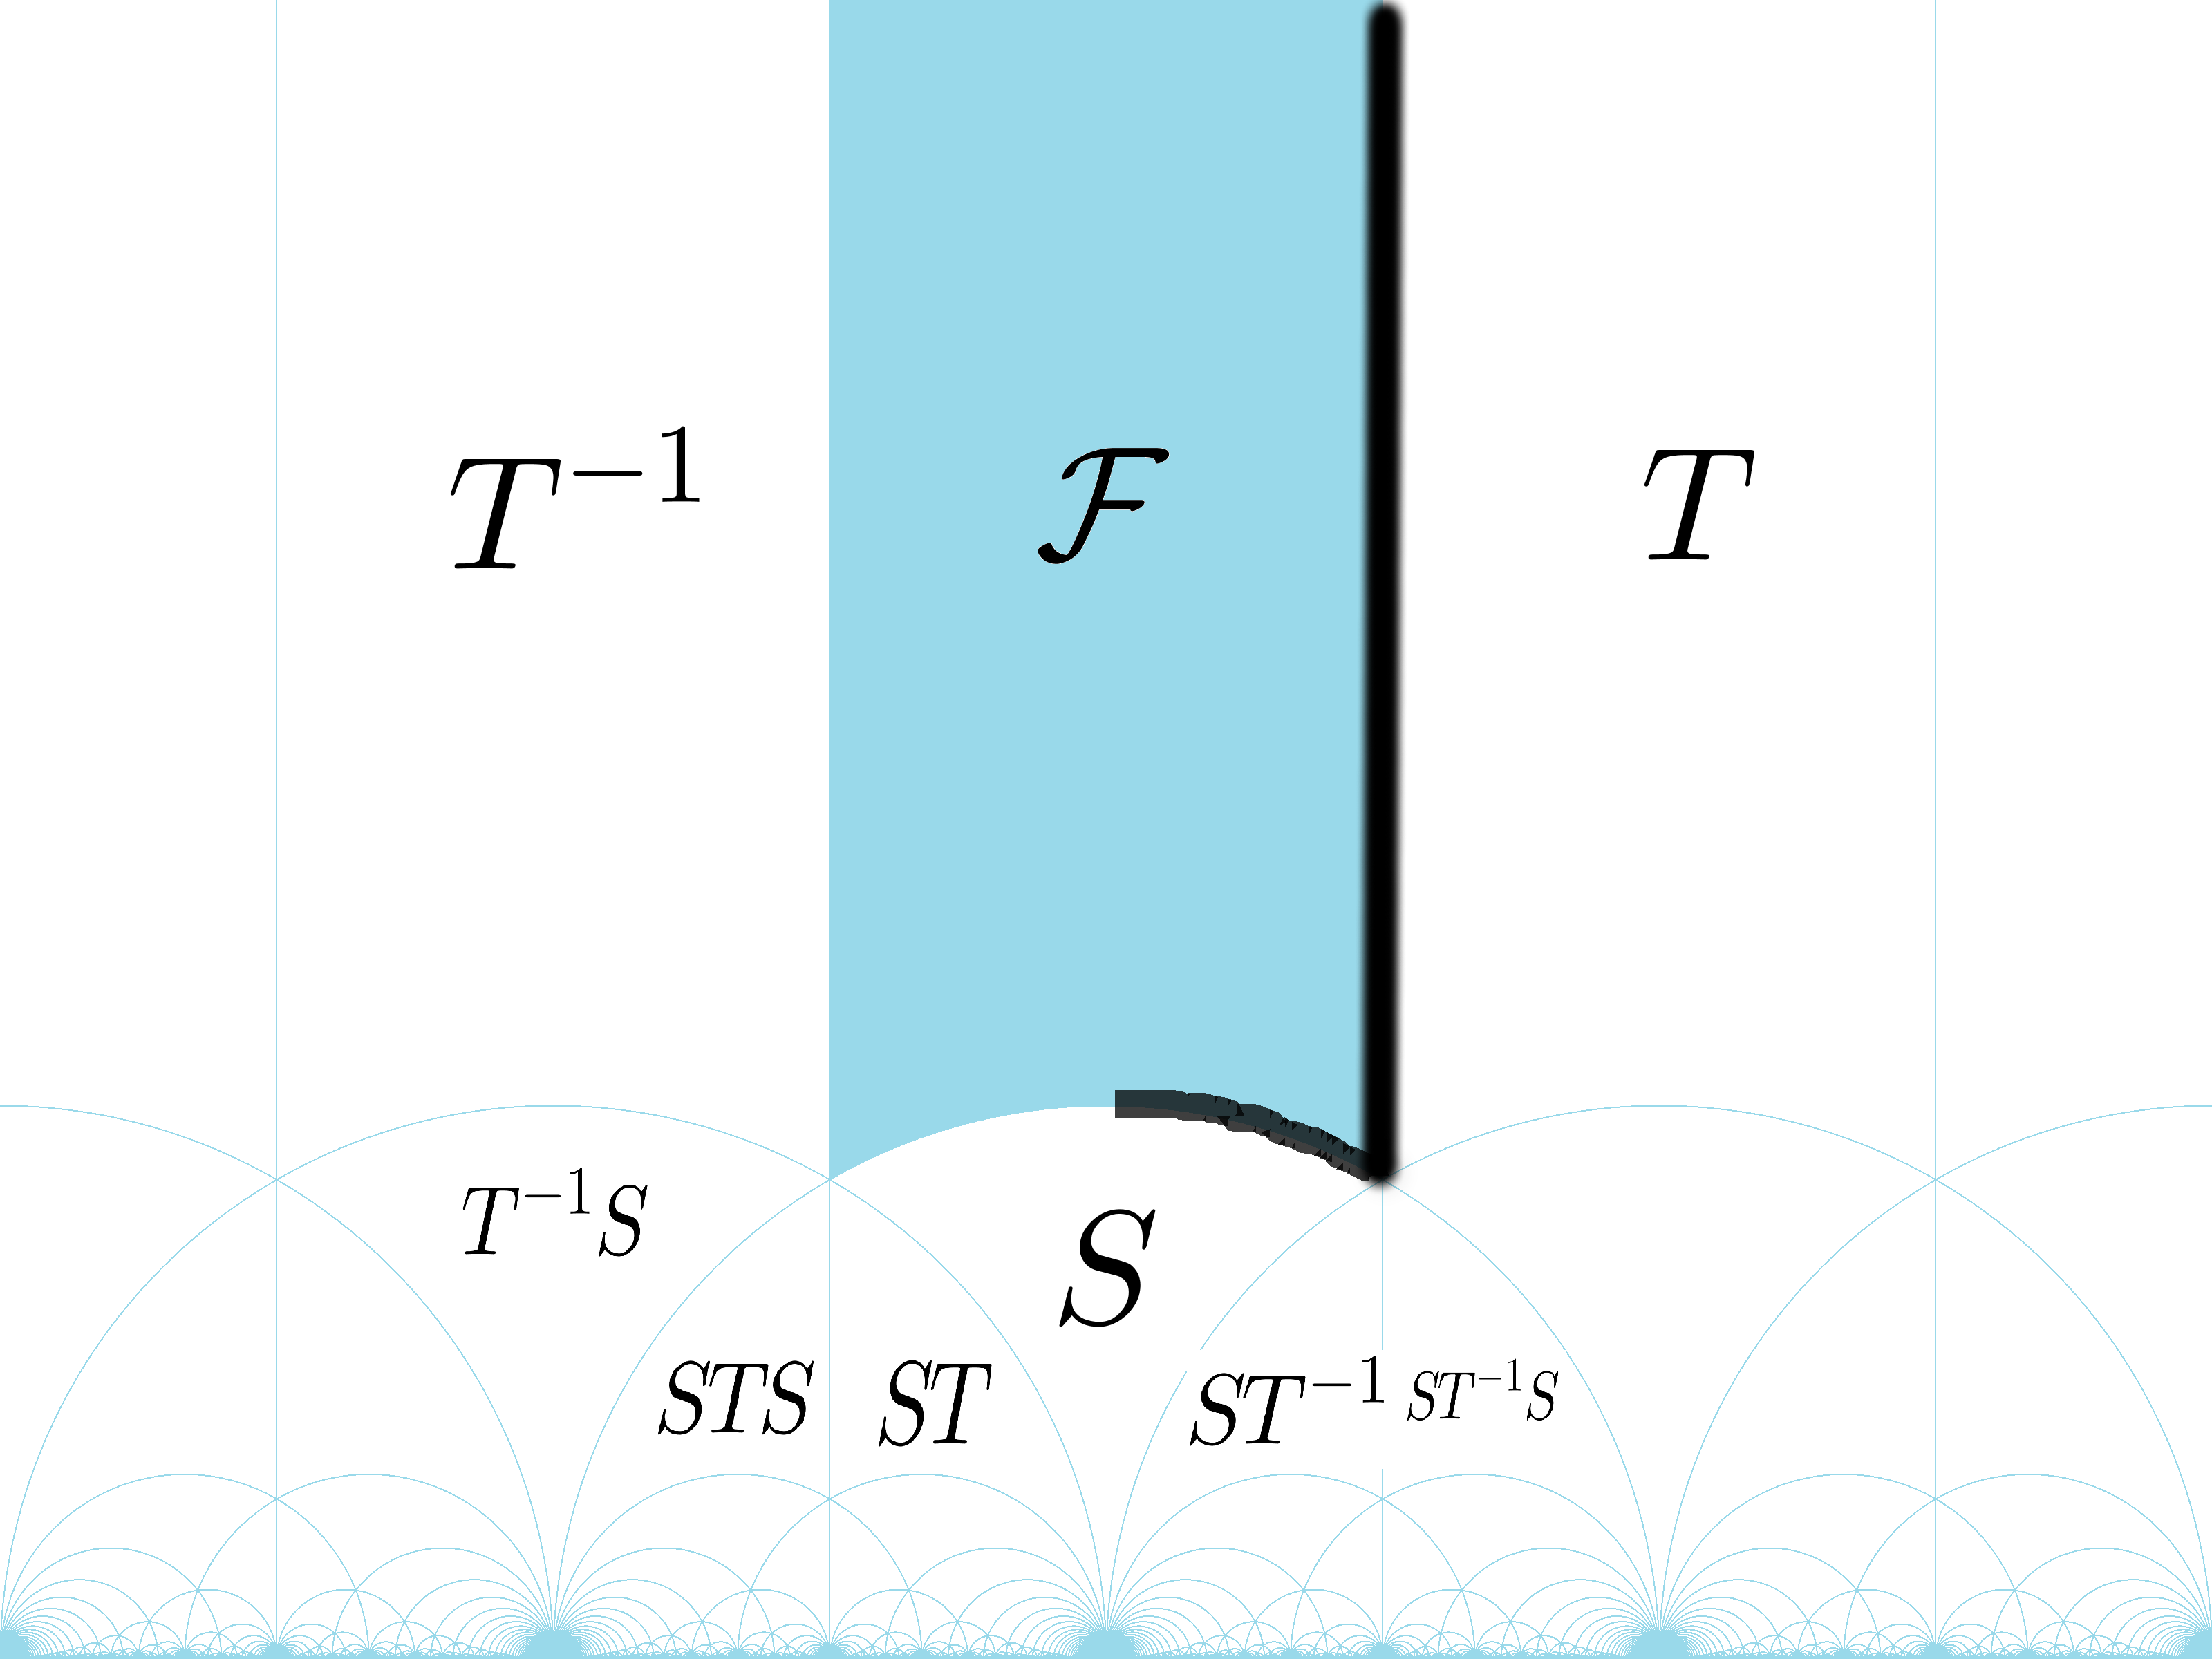
\includegraphics[scale=0.15]{modular3.png}
\caption{Domaine fondamental $\mathcal{F}$ du groupe modulaire et des images de $\mathcal{F}$ pour certains éléments de $\text{PSL}_2(\mathbb{Z})$.
 (Image de Arnaud Chéritat avec son autorisation)}
\label{neutre}
\end{figure}

\begin{proof}
On pose $\Gamma=\text{SL}_2(\mathbb{Z})$.
\begin{enumerate}
\item Posons $\tau=s+it \in \mathbb{H}$. En multipliant le numérateur et le dénominateur du quotient $\gamma\tau$ par $c\overline{\tau}$, nous trouvons
\begin{equation*}
\frac{a\tau+b}{c\tau+d}=\frac{ac|\tau|^2+(ad+bc)s+bd+(ad-bc)it}{|c\tau+d|^2}.
\end{equation*}
Nous avons alors 
\begin{equation} \label{equa2}
\Im\Big(\frac{a\tau+b}{c\tau+d}\Big)=\frac{(ad-bc)\Im(\tau)}{|c\tau+d|^2}=\frac{\Im(\tau)}{|c\tau+d|^2}
\end{equation}
qui est positive par la définition de $\mathbb{H}$. L'application est alors bien définie. On ne détaille pas ici les calculs pour montrer que c'est une action de groupe.
\\ \\
Les points a et b du lemme suivant montrent le point 2  du théorème et le point c démontre le point 3.
\newpage
\begin{lem}[\cite{ref21}] \label{leme1}
\begin{enumerate}
\item Pour tout $\tau \in \mathbb{H}$, l'orbite $\Gamma.\tau$ rencontre $\mathcal{F}'$.
\item Si $\tau$ et $\tau'$ deux points distincts de $\mathcal{F}'$ tels que $\Gamma.\tau=\Gamma.\tau'$ alors on a :  \begin{itemize}
\item soit $\Re(\tau)=\pm \frac{1}{2}$ et $\tau=\tau'\pm 1$,
\item soit $|\tau|=1$ et $\tau'=-\frac{1}{\tau}$.
\end{itemize}
 \item Si $\tau \in \mathcal{F}'$ alors le stabilisateur de $\tau$ dans $\Gamma$ est $\{ \pm 1\}$ sauf dans le cas où $\tau=i$ (resp. $\tau=e^{2i\pi/3}$ et $\tau=e^{i\pi/3}$) auquel cas le stabilisateur est engendré par $S$ (resp. $ST$).
\end{enumerate}
\end{lem}


\begin{proof}
\begin{enumerate}
\item
Soit $\tau \in \mathbb{H}$. La forme quadratique $q : \mathbb{R}^2 \rightarrow \mathbb{R}$, $(c,d) \mapsto |c\tau+d|^2$ est définie positive, alors $q$ admet un minimum sur $\mathbb{Z}^2 \backslash \{0\}$. D'après l'égalité (\ref{equa2}), on peut considérer l'ensemble $A=\{ \tau' \in \mathbb{H} : \Im(\tau') \hspace{0.2cm} \text{maximal} \} \subset \Gamma.\tau$. L'ensemble $A$ est invariant par $T$ de sorte qu'il existe $\tau' \in A$ tel que $|\Re(\tau')|\leqslant \frac{1}{2}$. Mais $-1/\tau' \in \Gamma.\tau$ et $\Im(-1/\tau')=\frac{\Im(\tau')}{|\tau'|^2}$ donc $|\tau'| \leqslant 1$. D'où $\tau '\in \Gamma.\tau \cap \mathcal{F}'$.
\item et (c)
Soient $\tau,\tau' \in \mathcal{F}'$ tels que $\Im(\tau') \geqslant \Im(\tau)$ et $\tau'=\gamma.\tau$ avec \\$\gamma =\begin{pmatrix} 
a & b \\
c & d 
\end{pmatrix} \in SL_{2}(\mathbb{Z})$.
Cela implique que $|c\tau+d| \leqslant 1$. Comme $|c\Im(\tau)| \leqslant 1$, alors $|c| \leqslant 1$.
Si $c=0$ alors $a=d=\pm 1$ et donc $\pm \gamma$ est une puissance de $T$ et on est dans le premier cas du lemme \ref{leme1} $(b)$.
Sinon, on peut supposer que $c=1$, quitte à remplacer $\gamma$ par $-\gamma$. Si $|\tau+d| \leqslant 1$ alors $|\tau|=1$. Les cas possibles sont alors :
\begin{enumerate}
\item $\tau \neq e^{2i\pi/3},e^{i\pi/3}$ et $d=0$.
Dans ce cas, $b=-1$ et $\tau'=a-1/\tau$ puis $a=0$ car $|\Re(-1/\tau)|<1/2$. Ainsi $\gamma=S$ et $\tau'=\tau=i$.
\item $\tau=e^{2i\pi/3}$ et $d=0,-1$. Si $d=0$, on a $b=-1$ et $\tau'=a-e^{-2i\pi/3}=a+e^{i\pi/3}$.
On a alors deux cas : soit $\tau'=e^{i\pi/3}, a=0$ et $\gamma\pm S$, soit $\tau'=\tau,a=-1$ et $\gamma=(ST)^2.$
\item Pour $\tau=e^{i\pi/3}$ et $d=0$ et $1$, la manière est identique que dans ii.
\end{enumerate}
\end{enumerate}
\end{proof}
\noindent On revient à la démonstration de la proposition \ref{modul}.
\item Les points a et b du lemme \ref{leme1} montrent que pour tout $\tau \in \mathbb{H}$, l'orbite $\Gamma.\tau$ rencontre $\mathcal{F}$ en un unique point d'où $\mathcal{F}$ est un domaine fondamental pour l'action de groupe de $\Gamma$ sur $\mathbb{H}$.
\item 
Soient $G$ le groupe engendré par $S$ et $T$, $\tau$ un point de l'intérieur de $\mathcal{F}'$ et $\gamma \in \Gamma$. D'après la démonstration du lemme \ref{leme1} point a, il existe $g \in G$ tel que $g^{-1}\gamma.\tau \in \mathcal{F}'$. Ainsi, $g^{-1}\gamma \in \Gamma$ fixe $\tau$ d'où $\tau=\pm 1$ par le lemme \ref{leme1} point c. D'où $\gamma \in G$ car $S^2=-\text{Id}_2 \in G$.
\end{enumerate}
\end{proof}

\begin{cor}[\cite{ref2}]
Tous les réseaux complexes $\Lambda$ sont homothétiques à\\$\Lambda_\tau=\mathbb{Z}+\mathbb{Z}\tau$ pour $\tau \in \mathcal{F}$.

\end{cor}
\noindent La preuve est admise.
\begin{definition}
\begin{enumerate}
\item
Une fonction méromorphe $f$ sur $\mathbb{H}$ est une \textbf{fonction modulaire} de poids $k$ si les deux conditions suivantes sont satisfaites : 
\begin{enumerate}
\item Pour tout $\gamma=\begin{pmatrix} 
a & b \\
c & d 
\end{pmatrix} \in SL_{2}(\mathbb{Z})$, $f(\tau)=(c\tau+d)^{-k}f(\gamma\tau)$.
\item La série de Fourier de $f$ en $q=e^{2i\pi\tau}$ est de la forme
\begin{equation*}
f(\tau)=\sum \limits_{n=n_{0}}^\infty c(n)q^n
\end{equation*}
pour $n_{0} \in \mathbb{Z}$.
\end{enumerate}
\item Une fonction modulaire $f$ est une \textbf{forme modulaire} de poids $k$ si $f$ est holomorphe sur $\mathbb{H}$ et $n_{0}=0$.
\end{enumerate}
\end{definition}

\noindent Avec les fonctions modulaires, nous pouvons démontrer le théorème d'uniformisation évoqué dans la remarque \ref{rem1}. 

\begin{theorem}[Uniformisation \cite{ref8}]
Soit $C$ une courbe elliptique de la forme de Weierstrass $y^2=x^3+ax+b$ telle que $4a^3+27b^2 \neq 0$. Il existe alors un unique réseau $\Lambda$ telle que $g_{2}(\Lambda)=60G_{4}(\Lambda)=-4a$, $g_{3}(\Lambda)=140G_{6}(\Lambda)=-4b$ et donc une bijection $\mathbb{C}/\Lambda \rightarrow C$.
\end{theorem}

\begin{proof}
Nous utiliserons le lemme suivant.
\begin{lem}[admis]\label{lem8}
Le $j$-invariant, défini dans la section I.4, est une fonction modulaire de poids 0
qui induit un isomorphisme entre $\mathbb{H}/PSL_{2}(\mathbb{Z})$ et $\mathbb{C}$.
\end{lem}

\noindent D'après l'identification vue dans le lemme \ref{lem8} et la remarque de la section "$j$-invariant", on peut choisir  $\tau \in \mathbb{H}$ tel que 
\begin{equation*}
j(\tau)=1728 \frac{4a^3}{4a^3+27b^2}=-1728 \frac{g_{2}(\tau)^3}{-g_{2}(\tau)^3+27g_{3}(\tau)^2}.
\end{equation*}
Ce qui revient aux égalités suivantes:
\begin{align*}
\frac{27b^2}{4a^3}=\frac{1728}{j(\tau)}-1&=-\frac{27g_{3}(\tau)^2}{g_{2}(\tau)^3} \\
\Bigg(\frac{b}{g_{3}(\tau)}\Bigg)^2 \Bigg(\frac{g_{2}(\tau)}{a}\Bigg)^3 &=-4.
\end{align*}
Posons 
\begin{equation*}
\alpha=\sqrt{\frac{ag_{3}(\tau)}{bg_{2}(\tau)}}
\end{equation*}
et $\Lambda=\alpha \Lambda_{\tau}= \alpha\tau\mathbb{Z}+\alpha\mathbb{Z}$.
Alors
\begin{align*}
g_{2}(\Lambda)&=\frac{g_{2}(\Lambda_{\tau})}{\alpha^4}=\frac{b^2g_{2}(\tau)^3}{a^2g_{3}(\tau)^2}=-4a
\\
g_{3}(\Lambda)&=\frac{g_{3}(\Lambda_{\tau})}{\alpha^6}=\frac{b^3g_{2}(\tau)^3}{a^3g_{3}(\tau)^2}=-4b
\end{align*}
De même, si $a=0$ alors $j(\tau)=g_{2}(\tau)=0$, et si $b=0$ alors $j(\tau)=1728$ et $g_{3}(\tau)=0$.
Dans les deux cas, il suffit de prendre
\begin{align*}
\alpha &=\sqrt[6]{\frac{g_{3}(\tau)}{-4b}} \hspace{2cm} \text{si} \hspace{0.2 cm} a=0 \\
\alpha &=\sqrt[4]{\frac{g_{2}(\tau)}{-4a}} \hspace{2cm} \text{si} \hspace{0.2 cm} b=0
\end{align*}
pour que $\Lambda=\alpha\Lambda_{\tau}$, ce qui démontre l'existence. \\
Démontrons l'unicité.
Supposons que 
\begin{equation*}
G_{4}(\Lambda_{1})=G_{4}(\Lambda_{2}) \hspace{2cm}
G_{6}(\Lambda_{1})=G_{6}(\Lambda_{2}).
\end{equation*}
Remarquons que $j(\Lambda_{1})=j(\Lambda_{2})$. 
D'après le théorème \ref{jinv}, les courbes elliptiques associées aux réseaux $\Lambda_1$ et $\Lambda_2$ sont isomorphes. D'après le corollaire \ref{cor2}, $\Lambda_1$ et $\Lambda_2$ sont homothétiques i.e il existe $\alpha \in \mathbb{C}$ tel que $\Lambda_{1}=\alpha\Lambda_{2}$. En utilisant l'égalité 
\begin{equation*}
G_{2k}(\alpha\Lambda)= \sum \limits_{\omega \in \Lambda'} \frac{1}{\alpha^{2k}\omega^{2k}}=
\alpha^{-2k}G_{2k}(\Lambda)
\end{equation*}
on a alors, par les hypothèses,
\begin{equation*}
G_{4}(\Lambda_{1})=G_{4}(\alpha\Lambda_{2})=\alpha^{-4}G_{4}(\Lambda_{2})=G_{4}(\Lambda_{2})
\end{equation*}
d'où $\alpha^4=1$. De même, en utilisant $G_{6}(\Lambda_{1})=G_{6}(\Lambda_{2})$, on a $\alpha^6=1$. \\
On conclut la démonstration avec $\alpha^2=1$ i.e $\alpha=\pm 1$ et $\Lambda_{1}=\pm \Lambda_{2}=\Lambda_{2}$.
\end{proof}


\noindent On a vu que le $j$-invariant permet de classifier les courbes elliptiques mais il est possible de le faire avec les réseaux du plan.

\begin{theorem}[\cite{ref28}] \label{theo10}
Soit $\mathscr{R}$ l'ensemble des réseaux de $\mathbb{C}$ (c'est-à-dire les sous-groupes de $\mathbb{C}$ isomorphes à $\mathbb{Z}^2$ non contenus dans une droite réelle).
On a alors l'équivalence $\mathscr{R}/\mathbb{C}^* \cong \mathbb{H} /SL_{2}(\mathbb{Z})$ qui permet d'identifier $\mathscr{R}/\mathbb{C}^*$ aux classes d'isomorphisme des courbes elliptiques.
\begin{equation*}
 \xymatrix{
    \mathscr{R} \ar[r] \ar[d]  & \mathbb{H} \ar[d] \\
    \mathscr{R}/\mathbb{C}^* \eq[r] & \mathbb{H} /SL_{2}(\mathbb{Z})
  }
 \end{equation*}
\end{theorem}


\begin{proof}
On note $M$ l'ensemble des couples $(\omega_{1},\omega_{2}) \in \mathbb{C}^* \times \mathbb{C}^*$ tels que \\ $\Im(\omega_{1}/\omega_{2})>0$.
Soit l'application 
\begin{align*}
\pi : M &\rightarrow \mathbb{H} \\
(\omega_{1},\omega_{2}) &\mapsto \frac{\omega_{1}}{\omega_{2}}
\end{align*}
D'une part, $\pi$ est surjective par la définition de $\mathbb{H}$.
D'autre part, $\pi(\omega_{1},\omega_{2})=\pi(\omega'_{1},\omega'_{2})$ si et seulement si il existe $\lambda$ non nul tel que $(\omega_{1},\omega_{2})=\lambda(\omega'_{1},\omega'_{2})$.
L'application $\pi$ induit alors par passage au quotient une bijection $M/\mathbb{C}^* \rightarrow \mathbb{H}$.\\
Posons l'application 
\begin{align*}
\Lambda : M &\rightarrow \mathscr{R} \\
(\omega_{1},\omega_{2}) &\mapsto \omega_{1}\mathbb{Z}+\omega_{2}\mathbb{Z}.
\end{align*}
L'application $\Lambda$ est surjective. En effet, prenons un réseau $\omega_{1}\mathbb{Z} + \omega_{2}\mathbb{Z}$, quitte à changer $\omega_{2}$ en $-\omega_{2}$, on peut supposer que $\Im(\omega_{1}/\omega_{2})\geqslant 0$ d'où la surjectivité.
On veut montrer que $M/SL_{2}(\mathbb{Z}) \cong \mathscr{R}$. On utilise l'action de groupe suivant
\begin{align*}
\text{SL}_{2}(\mathbb{Z}) \times M &\rightarrow M \\
\Big(
  \left( {\begin{array}{cc}
   a & b \\
   c & d \\
  \end{array} } \right) ,
  (\omega_{1},\omega_{2}) \Big) &\rightarrow (a\omega_{1}+b\omega_{2}, c\omega_{1}+d\omega_{2}).
\end{align*}
Soit $R=\omega_{1}\mathbb{Z} + \omega_{2}\mathbb{Z}$ un réseau avec $(\omega_{1},\omega_{2})$. Alors, $(\omega'_{1},\omega'_{2}) \in \mathbb{Z}^2$ est une base de $R$ si et seulement si il existe $g \in \text{GL}_{2}(\mathbb{Z})$ tel que $g(\omega_{1},\omega_{2})=(\omega'_{1},\omega'_{2})$. Quitte à changer $\omega'_{2}$ en $-\omega'_{2}$, on peut supposer $(\omega'_{1},\omega'_{2}) \in M$. Si $g \in \text{GL}_{2}$ (de déterminant $\pm 1$ puisque inversible) vérifie $g(\omega_{1},\omega_{2})=(\omega'_{1},\omega'_{2})$ alors le signe de $\Im(\omega'_{1}/\omega'_{2})$ est le signe de $\Im(\omega_{1}/\omega_{2})$ fois det($g$). Donc det($g$)>0 d'où $g \in \text{SL}_{2}(\mathbb{Z})$. \\
On a alors montré que $(\omega'_{1},\omega'_{2}) \in \mathbb{Z}^2$ est une base de $R$ si et seulement si il existe $g \in \text{SL}_{2}(\mathbb{Z})$ tel que $g(\omega_{1},\omega_{2})=(\omega'_{1},\omega'_{2})$.
Autrement dit, $\Lambda$ induit un isomorphisme $M/\text{SL}_{2}(\mathbb{Z}) \cong \mathscr{R}$. 
 Comme $\text{SL}_{2}(\mathbb{Z}) \subset \text{GL}_{2}(\mathbb{Z})$ agit de façon $\mathbb{C}$-linéaire, les actions de groupes $\mathbb{C}^*$ et $\text{SL}_{2}(\mathbb{Z})$ sur $M$ commutent. Or on a prouvé que $M/\mathbb{C}^* \cong \mathbb{H}$ d'où 
 \begin{equation*}
 (M/\text{SL}_{2}(\mathbb{Z}))/\mathbb{C}^*=(M/\mathbb{C}^*)/\text{SL}_{2}(\mathbb{Z})
 \end{equation*}
,ce qui  nous donne l'isomorphisme $\mathscr{R}/\mathbb{C}^* \cong \mathbb{H} /\text{SL}_{2}(\mathbb{Z})$. 
\end{proof}




\subsection{Multiplication complexe}
\noindent Par le théorème \ref{theo7}, End($C$) est identifié à l'ensemble $\{\alpha \in \mathbb{C} : \alpha \Lambda=\Lambda\}$. L'anneau End($C$) est alors un sous-anneau de $\mathbb{C}$ d'où $\mathbb{Z} \subset$ End($C$).
Nous avons vu la notion d'isogénie dans la section précédente et on sait que chaque courbe elliptique contient l'isogénie multiplicative $[n]$ définie dans la section I.3. Pour la plupart des courbes elliptiques, il n'y a pas d'autres isogénies, mais nous nous intéressons dans cette section aux courbes elliptiques munies d'autres isogénies.


\begin{definition}
Si $C$ est une courbe elliptique, on dit que $C$ est munie d'une \textbf{multiplication complexe} si End($C$) est plus grand que $\mathbb{Z}$, i.e il existe un endomorphisme autre que $[n]$.
\end{definition}

\begin{ex}[\cite{ref}]
\normalfont Soit $C$ la courbe elliptique suivante : $C :y^2=x^3+x$.
Elle possède la multiplication complexe
\begin{equation*}
\phi(x,y)=(-x,iy).
\end{equation*}
On pourra montrer que $(-x,iy) \in C$ et que $\phi^2(P)=-P$.
\end{ex}


\noindent Le résultat suivant est le théorème clé de la section : il permet de caractériser la multiplication complexe avec les extensions quadratiques.


\begin{theorem} [\cite{ref24}] \label{theoo1}
Soit $C$ une courbe elliptique et $\Lambda=\tau \mathbb{Z}+\mathbb{Z}$ son réseau correspondant.
Si la courbe $C$ possède une multiplication complexe alors $\tau \in \mathbb{Q}(\sqrt{-d})$ avec $d \in \mathbb{N}^*$.
L'anneau End(C) est alors un sous-anneau des entiers de $\mathbb{Q}(\sqrt{-d})$. La réciproque est vraie, 
si $\tau=r+s\sqrt{-d} \in \mathbb{Q}(\sqrt{-d})$ alors la courbe $C$ est munie une multiplication complexe. \\
 Dans ce cas,
\begin{equation*}
End(C)=\{\alpha+\beta\tau : \alpha,\beta \in \mathbb{Z} \hspace{0.3cm} et \hspace{0.3cm} 2\beta r,\beta (r^2+ds^2)\in \mathbb{Z} \}.
\end{equation*}
\end{theorem}

\begin{proof}
Prouvons le sens direct.
Par le théorème \ref{theo7}, nous allons déterminer End($C$) comme l'ensemble $A=\{\alpha \in \mathbb{C} : \alpha \Lambda \subset \Lambda \}$.
Pour que $\alpha \in A$, il faut et il suffit qu'il existe $a,b,c,e \in \mathbb{N}$ tel que
\begin{align*}
\alpha &=a+b\tau \\
\alpha \tau&=c+e\tau
\end{align*}
D'une part, si $\alpha \in \mathbb{R}$ alors $\alpha \in \mathbb{Z}$ car $\Im(\tau)>0$. D'où End($C$) $\cap \hspace{0.1cm} \mathbb{R}= \mathbb{Z}$.  \\
D'autre part, si $C$ a une multiplication complexe alors il existe $\alpha \in \mathbb{C} \backslash \mathbb{R}$, i.e $b \neq 0$.
En éliminant $\alpha$, nous obtenons
\begin{equation*}
b\tau^2+(a-e)\tau-c=0
\end{equation*}
$\tau$ est alors une extension quadratique de $\mathbb{Q}$. Comme $\Im(\tau) >0$, c'est une extension quadratique imaginaire d'où il existe $d \in \mathbb{N}^*$ tel que $\tau \in \mathbb{Q}(\sqrt{-d})$. \\
De même, en éliminant $\tau$,
\begin{equation*}
\alpha^2-(a-e)\alpha+(ae-bc)=0
\end{equation*}
alors $\alpha$ est un élément entier sur $\mathbb{Z}$ , ce qui conclut la première partie de la démonstration.
Maintenant, supposons que $\tau=r+s\sqrt{-d} \in \mathbb{Q}(\sqrt{-d})$. Par le théorème \ref{theo7}, End($C$) est l'ensemble des $\alpha=a+b\tau$ , $a,b \in \mathbb{Z}$ tels que $\alpha \tau \in \Lambda$.
En multipliant par $\tau$, i.e $\alpha \tau=a\tau+b\tau^2,$ il faut que $b\tau^2 \in \Lambda$. \\
 Par ailleurs, 
\begin{equation*}
\tau^2=r^2-ds^2+2rs\sqrt{-d}=2r\tau-(r^2+ds^2).
\end{equation*}
Ainsi, il est nécessaire et suffisant d'avoir $2br \in \mathbb{Z}$ et $b(r^2+ds^2) \in \mathbb{Z}$. \\
En particulier, End($C$) $\not \cong \mathbb{Z}$, ce qui conclut la démonstration.
\end{proof}

\begin{cor} [\cite{ref24}]
Il y a un nombre dénombrable de $j \in \mathbb{C}$
tel que la courbe elliptique associée soit munie d'une multiplication complexe.
\end{cor}

\begin{proof}
En effet, il y a un nombre dénombrable d'extensions quadratiques de $\mathbb{Q}$.
\end{proof}
\noindent En clair, il existe peu de courbes elliptiques munies d'une multiplication complexe. La plupart du temps, End$(C) \cong \mathbb{Z}$.
\begin{ex}[\cite{ref24}]
\begin{enumerate}
\item
\normalfont Prenons $\tau=i$ alors End($C$) est l'anneau des entiers de Gauss $\mathbb{Z}[i]$, par le théorème \ref{theoo1}.
Le groupe des unités End($C)^*$ est $\{\pm 1,\pm i\}$, groupe cyclique d'ordre 4 donc isomorphe à $\mathbb{Z}/4\mathbb{Z}$. Comme Aut($C$) est d'ordre 4, par le corollaire \ref{corol2}, son $j$-invariant est 1728. Une autre manière de le voir est par le réseau $\Lambda=\mathbb{Z}+i\mathbb{Z}$ et que
\begin{equation*}
g_{3}=140 \sum \limits_{\omega \in \Lambda'} \frac{1}{\omega^6}=140 \sum \limits_{\omega \in \Lambda'} \frac{1}{(i\omega)^6}=-g_{3}
\end{equation*}
Ce qui implique $g_{3}=0$.
L'équation de $C$ est de la forme $y^2=x^3-b$.
\item Pour $\tau=\rho$ où $\rho^3=1$. Dans ce cas, End($C$)=$\mathbb{Z}[\rho]$, i.e l'anneau des entiers $\mathbb{Q}(\sqrt{-3})$. Comme End($C)^*=\{\pm 1,\pm \rho,\pm \rho^2 \} \cong \mathbb{Z}/6\mathbb{Z}$, $j=0$ par le corollaire \ref{corol2}. L'équation est alors $y^2=x^3-b$.
\end{enumerate}
\end{ex}













\begin{rem}[\cite{ref2}]
\normalfont Notre étude des courbes elliptiques sur $\mathbb{C}$ se généralise sur des corps algébriquement clos de caractéristiques 0, c'est le principe de Lefschetz. 
\end{rem}










\newpage

\newpage

\appendix

\newpage
\section{Bibliographie} 
\bibliographystyle{alpha}
\bibliography{rational}
\nocite{ref11}
\nocite{ref16}
\nocite{ref21}
\nocite{ref27}
\newpage
\section{Annexe}
\textbf{I.1 Loi de groupe}
\begin{figure}[!h]
\centering
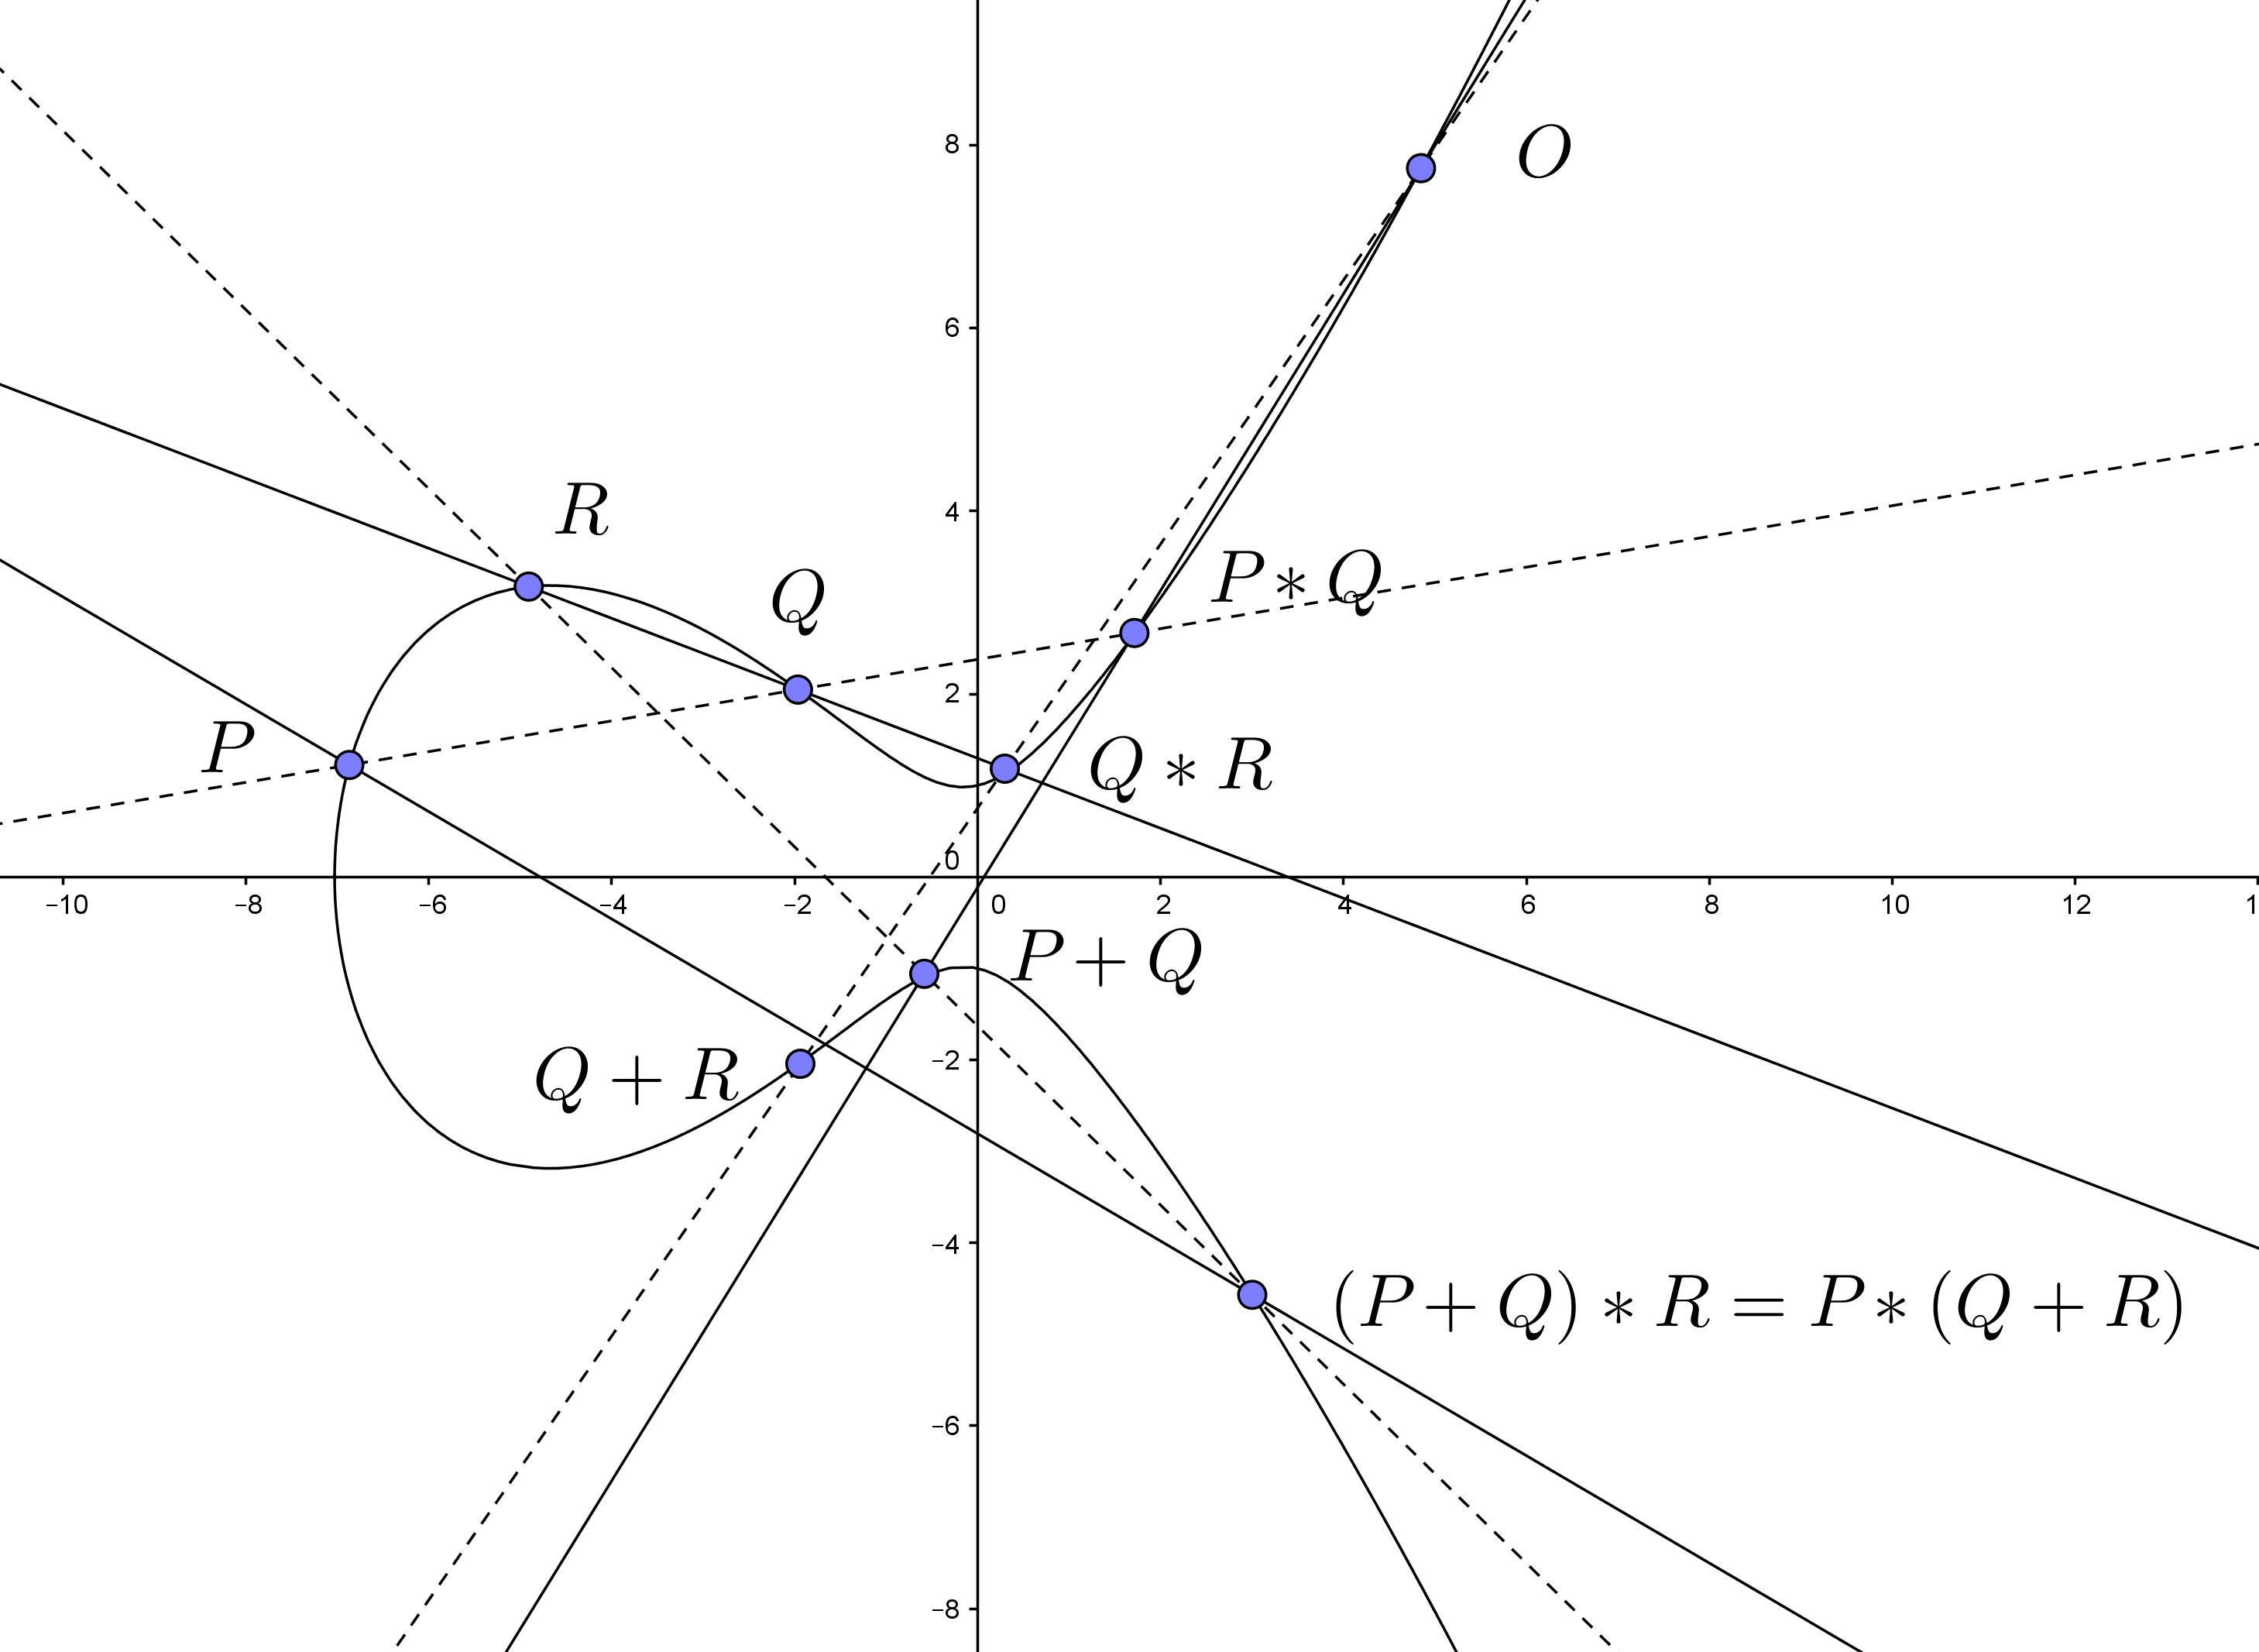
\includegraphics[scale=0.18]{associativite.png}
\caption{Associativité}
\label{neutre}
\end{figure}
\newpage
khhhhhhhhhhhhhhhhhhhhhh
\addcontentsline{toc}{section}{\protect\numberline{C}Programmes Maple}


\end{document}
